\clearpage



\section{矩阵的运算}

\subsection{矩阵的加法、数乘和乘法}

\subsubsection{基本性质}

本节我们讨论矩阵加法、数乘和矩阵乘法三种运算.
掌握这三种运算规则本身并不困难，
关键是要理解它与线性映射的加法、数乘和复合运算之间的联系.
本节不涉及线性空间的基变换，
因此在这里讨论矩阵运算和线性映射运算原则上没什么区别.
但为了显示这两个概念的区分，
我们把线性映射用大写花体字母表示（如$\mathcal{A},\mathcal{B}$），
其表示矩阵仍用普通的大写字母表示（如$A,B$）.
考虑到相同数域上$n$维线性空间皆同构，
方便起见，
本节用$\mathbb{K}^n$代替数域$\mathbb{K}$上一般的$n$维线性空间.


矩阵乘法是对线性映射复合的表示.
首先要注意不是任意两个矩阵之间都允许做乘法，
必须是\textbf{前一个矩阵的列数等于后一个矩阵的行数}，
即$m \times n$矩阵与$n \times s$矩阵可以做乘法.
这是因为在映射的复合中，前一个映射的陪域应当等于后一个映射的定义域，
即$\mathbb{K}^s \to \mathbb{K}^n$的线性映射复合一个
$\mathbb{K}^n \to \mathbb{K}^m$的线性映射是允许的.

映射的复合满足结合律，但是一般不可交换——
即使交换复合顺序之后依然是合法的，
它与换序之前也未必相同.
因此，可以断言\textbf{矩阵乘法满足结合律}，
即$A(BC) = (AB)C$总是成立；
但\textbf{矩阵乘法不满足交换律}.
即$AB \ne BA$是很有可能发生的（即使$A$和$B$是同阶的方阵）.

在做矩阵计算时，
如果不知道$A$和$B$的确切身份，
应当默认$AB$不能转化成$BA$.
初学者在这里常常会犯错.
例如计算$(A+B)^2$，
或许顺手就把它展开成$A^2 + 2AB + B^2$，
但实际上$(A+B)^2 = (A+B)(A+B) = A^2 + AB + BA + B^2$，
一般不等于$A^2 + 2AB + B^2$.
又如$(AB)^2$，
应当是$ABAB$而不等写成$A^2 B^2$.\vspace{0.5em}

但是，
$AB \ne BA$也不是任何情况下都不对.
最简单的例子就是单位矩阵$I_n$.
我们曾介绍过，
它是代表恒等映射的矩阵，
它在矩阵乘法中的作用如同“$1$”在实数乘法中的作用，
即满足：

\begin{eq1}
    I_n A_n = A_n I_n = A_n  \\[12pt]
\end{eq1}

由此还发现，
对任意的$k \in \mathbb{K}$，
有：

\begin{eq1}
    (kI_n) A_n = A_n (kI_n) = kA_n  \\[12pt]
\end{eq1}

即单位矩阵的$k$倍$kI_n$也与任何同阶方阵可交换，
且乘法的效果等同于数乘$k$.
因此$kI_n$也称为\textbf{数量矩阵}.
处理只涉及数乘、单位矩阵和一个未知矩阵$A$的矩阵代数式时，
就不必畏手畏脚，
可以验证我们熟知的一些代数恒等式代入矩阵后依然成立，
例如运用立方差公式有：

\begin{eq1}
    I-A^3 = (I-A)(I + A + A^2) \\[12pt]
\end{eq1}
初学者有时会因为太害怕交换律不成立而做不出这种最简单的因式分解.
这种极端也要通过练习尽量地避免.

讲到这里，
你可能想问：“一般情况下，两个矩阵的乘法到底什么时候可以互换？”
很遗憾，
凭借线性代数的课内知识是回答不了这个问题的.
我也没有在讲义中解答这个问题的计划.
不过随着学习的深入我们将有能力给出矩阵乘法交换的一些充分条件.
目前，
我们只要对矩阵乘法的交换保持足够的警惕就可以了.

最后，
因为矩阵的行列式表示线性映射的体积伸缩比例，
连续两个线性映射的伸缩比例相乘，
应该得到总的伸缩比例.
因此，
自然地有行列式在矩阵乘法下的公式：
$|AB| = |A||B|$.


\subsubsection{矩阵运算与秩}

本节我们讨论矩阵的秩在矩阵运算下的变换规律.
主要关注矩阵加法和矩阵乘法.
请注意，
我们不是要从矩阵本身的计算来看待这些规律，
而是要从线性空间和线性映射的角度提供一个更本质的理解.
要想真正取得这种理解（或者你希望在解题时灵活运用这种理解），
必须牢记以下的基本事实.
首先，\textbf{一个线性映射的像空间的维数即是其表示矩阵的秩}，
即$\mathrm{rank} (A) = \dim \operatorname{Im} \mathcal{A}$.
这一点在讲义第二章中是以定义的方式提出来的.
另外，
对于$\mathcal{A}: \mathbb{K}^n \to \mathbb{K}^m$，
有维数公式$n = \mathrm{rank}(A) + \dim W$，
其中$W$是指齐次线性方程组$A\bm{X} = \bm{0}$的解空间.
用线性映射的语言，
维数公式可以改写成$n = \dim \operatorname{Im} \mathcal{A} + \dim \operatorname{Ker} \mathcal{A} $.
\vspace{1em}

对于矩阵加法的秩，
有一个重要的不等式：

\begin{eq1}
    \mathrm{rank}(A+B) \leq \mathrm{rank}(A) + \mathrm{rank}(B)
\end{eq1}

换而言之：
\begin{eq1}
    \dim \operatorname{Im} (\mathcal{A}+\mathcal{B})
    \leq
    \dim \operatorname{Im} \mathcal{A} +
    \dim \operatorname{Im} \mathcal{B}   
\end{eq1}

从这个角度来看，
上述秩不等式是在讨论$\operatorname{Im} (\mathcal{A}+\mathcal{B})$与
$\operatorname{Im} \mathcal{A}, \operatorname{Im} \mathcal{B}$这三个线性子空间的维数关系.
它们之间有一个直接的关系是：

\begin{eq1}
    \operatorname{Im}(\mathcal{A} + \mathcal{B})
    \subset
    \operatorname{Im} \mathcal{A} + \operatorname{Im} \mathcal{B}
\end{eq1}
这是因为$\operatorname{\mathcal{A} + \mathcal{B}}$中的元素必定形如
$\mathcal{A}\bm{x} + \mathcal{B}\bm{x}$.
于是我们立即得到：

\begin{eq1}
    \dim \operatorname{Im}(\mathcal{A} + \mathcal{B})
    \leq
    \dim (\operatorname{Im} \mathcal{A} + \operatorname{Im}\mathcal{B})
    \leq
    \dim \operatorname{Im} \mathcal{A} + \dim \operatorname{Im} \mathcal{B}
\end{eq1}
其中，第一个不等号是从包含关系得到的；
第二个不等号是从子空间加法的维数公式得到的.
不妨在此回忆一下这个公式：

\begin{eq1}
    \dim (V_1) + \dim (V_2) = \dim (V_1 + V_2) + \dim (V_1 \cap V_2)
\end{eq1}

这个不等式到此就证明完毕了.
对于不熟悉线性映射语言的同学，
可能更期望一种纯矩阵运算的证明.
为此我们稍微多做一些讨论.
在维数公式中，
$\dim (V_1) + \dim (V_2)$也是有一定意义的，
它其实就是直和空间$V_1 \oplus V_2$的维数.
回到刚才的不等式，
所谓$\mathrm{rank}(A) + \mathrm{rank}(B)$，
或者$\dim \operatorname{Im}\mathcal{A} + 
\dim \operatorname{Im}\mathcal{B}$，
实际上是指$\dim (\operatorname{Im}\mathcal{A}  \oplus \operatorname{Im}\mathcal{B})$.
我们知道这其实是一个分块对角矩阵的秩：

\begin{eq1}
    \begin{pmatrix}
        A & O \\[4pt]
        O & B
    \end{pmatrix} \\[12pt]
\end{eq1}

它代表一个$\mathbb{K}^n \oplus \mathbb{K}^n  \to \mathbb{K}^m \oplus \mathbb{K}^m$
的线性映射，$\mathcal{A}$是它在第一个$\mathbb{K}^n$上的限制，
$\mathcal{B}$是它在第二个$\mathbb{K}^n$上的限制.
$\operatorname{Im}\mathcal{A} \oplus \operatorname{Im}\mathcal{B}$
即是它的像空间.
当然，
也不难用纯矩阵的方法证明（见习题部分）：

\begin{eq1}
    \mathrm{rank}
    \begin{pmatrix}
        A & O \\[4pt]
        O & B
    \end{pmatrix}
    = 
    \mathrm{rank}(A) + \mathrm{rank}(B)\\[12pt]
\end{eq1}

利用分块矩阵的初等变换，
（后文将会提及），
我们将能证明：

\begin{eq1}
    \mathrm{rank}
    \begin{pmatrix}
        A & O \\[4pt]
        O & B
    \end{pmatrix}
    = 
    \mathrm{rank}
    \begin{pmatrix}
        A & O \\[4pt]
        B & B
    \end{pmatrix}
    = 
    \mathrm{rank}
    \begin{pmatrix}
        A+B & B \\[4pt]
        B & B
    \end{pmatrix}
    \geq
    \mathrm{rank}(A+B) \\[12pt]
\end{eq1}

于是，
通过分块矩阵处理两个矩阵秩的相加，
我们用纯矩阵的方式再次证明了这个不等式.
出于考试的目的，
同学们应该熟悉这两种思路中的至少一种.
\vspace{1em}

对于矩阵乘法的秩，
也有一个重要的不等式：

\begin{eq1}
    \mathrm{rank}(AB)
    \leq
    \min \{ \mathrm{rank}(A) , \mathrm{rank}(B) \}
\end{eq1}

从矩阵运算的角度讲，
这意义已经很明确：
\textbf{矩阵乘法不会使得矩阵的秩增大.}
现在从线性映射的角度给予证明，
并揭示更深刻的意义.
设$A$和$B$分别是$m \times n$和$n \times s$矩阵，
对应的线性映射$\mathcal{A}: \mathbb{K}^n \to \mathbb{K}^m$和
$\mathcal{B}: \mathbb{K}^s \to \mathbb{K}^n$.
其复合映射$\mathcal{A} \circ \mathcal{B} : \mathbb{K}^s \to \mathbb{K}^m$，
$AB$即是它的表示矩阵.

先证明$\mathrm{rank}(AB) \leq \mathrm{rank}(A)$.
即$\dim \operatorname{Im}(\mathcal{A} \circ \mathcal{B}) \leq \dim \operatorname{Im}\mathcal{A}$.
这其实是很简单的事实.
如图所示，
$\operatorname{\mathcal{A} \circ \mathcal{B}}$实质上是
对$\mathbb{K}^s$先作用$\mathcal{B}$，
映射到像空间$\operatorname{Im}\mathcal{B}$上，
再被$\mathcal{A}$作用得到的.
因此，
所谓$\operatorname{Im}(\mathcal{A} \circ \mathcal{B})$，
其实就是$\mathcal{A}$在$\operatorname{Im}\mathcal{B}$上的限制的像空间，
即$\operatorname{Im}(\mathcal{A}|_{\operatorname{Im}\mathcal{B}})$.
这显然包含于未限制定义域的像空间$\operatorname{Im}\mathcal{A}$，
维数当然不会超过它.

再来证明$\mathrm{rank}(AB) \leq \mathrm{rank}(B)$.
即$\dim \operatorname{Im}(\mathcal{A}|_{\operatorname{Im}\mathcal{B}}) \leq \dim \operatorname{Im} \mathcal{B} $.
对$\mathcal{A}|_{\operatorname{Im}\mathcal{B}}$列出维数公式（注意定义域是$\operatorname{Im}\mathcal{B}$），
便会发现这是显然的：

\begin{eq1}
    \dim \operatorname{Im}\mathcal{B}
    = 
    \dim \operatorname{Im}(\mathcal{A}|_{\operatorname{Im}\mathcal{B}})
    + \dim \operatorname{Ker}(\mathcal{A}|_{\operatorname{Im}\mathcal{B}})
\end{eq1}

你可以看到，
这个证明过程中并不涉及一丁点真正的计算，
只是对复合映射$\mathcal{A} \circ \mathcal{B}$中涉及的子空间维数进行了粗浅的分析而已.
这个不等式实际上蕴含两条关于线性映射的知识：
第一，
\textbf{复合映射$\mathcal{A} \circ \mathcal{B}$的像空间即是
$\mathcal{A}$限制在$\operatorname{Im}\mathcal{B}$上的像空间.}
第二，
\textbf{一个线性映射的像空间维数不能超过其定义域的维数.}



\subsection{可逆矩阵与初等变换}

\subsubsection{可逆矩阵的性质}

可逆矩阵所表示的线性映射的双射，
即线性同构映射.
在前几章中已经充分讨论了可逆矩阵的性质，
这里只举几点最重要的.
\textbf{一个矩阵可逆当且仅当它满秩}.
关于行列式，
则有$|A^{-1}| = |A|^{-1}$.
最后，
\textbf{一个矩阵与可逆矩阵相乘不改变秩.}
具体来说，
设$P_{m \times m}$和$Q_{n \times n}$是可逆矩阵，
$A_{m \times n}$的秩为$r$，
则有：
\begin{eq1}
    \mathrm{rank}(PA) = \mathrm{rank}(AQ) = \mathrm{rank} (PAQ) = r
\end{eq1}


\subsubsection{初等变换与初等矩阵}

回顾矩阵等价的性质.
我们知道，
$A_{m \times n}$与$B_{m \times n}$等价，
当且仅当$\mathrm{rank}(A) = \mathrm{rank}(B)$.
对于等价变换的理解有两种.
第一种正如上一小节所说，
如果$A$的左右各乘一个可逆矩阵之后得到$B$，
则$A$与$B$等价.
第二种是，
如果$A$能通过初等行变换和初等列变换得到$B$，
则$A$与$B$等价.
我们不免会想，
可逆矩阵乘法与初等变换之间一定存在某种关联.

我们定义，
由单位矩阵$I$经过一次初等行（列）变换得到的矩阵称为\textbf{初等矩阵}.
分为三种：
\vspace{0.5em}

(1)~
把$I$的第$i$行的$k$倍加到第$j$行上
（或者等价地，第$j$列的$k$倍加到第$i$行上），
得到的初等矩阵记为$P(j,i(k))$.

(2)~交换$I$的第$i$行和第$j$行
（或者等价地，交换第$i$列和第$j$列），
得到的初等矩阵记为$P(i,j)$.

(3)~把$I$的第$i$行乘以非零常数$c$
（或者等价地，把第$i$列乘以非零常数$c$），
得到的初等矩阵记为$P(i(c))$.

\vspace{0.5em}


可以直接验证，
全部三种初等矩阵都一定是可逆的.
而且，
\textbf{
用初等矩阵左乘一个任意矩阵$A$，
相当于对$A$进行了一次相应的初等行变换；
用初等矩阵右乘一个任意矩阵$A$，
相当于对$A$进行了一次相应的初等列变换.}
这样一来，
我们就用矩阵乘法的方式实现了对矩阵的初等变换.
这一点在矩阵求逆问题中是特别实用的.
要想直接计算一个可逆矩阵$A$的逆矩阵很困难
（比如用伴随矩阵法，需要计算$n^2$个$n-1$阶代数余子式），
但是将$A$初等变换为一个单位矩阵总是可以做到的.
假如我们只使用一系列初等行变换，
将$A$变成了单位矩阵$I$，
这相当于对$A$左乘了一系列初等矩阵$P_1 , P_2, \cdots ,P_k$：

\begin{eq1}
    (P_k P_{k-1} \cdots P_2 P_1) A = I
\end{eq1}

则这些初等矩阵的乘积
$P_k P_{k-1} \cdots P_2 P_1$
就是$A^{-1}$.
换句话说，
把这一系列初等行变换作用到$I$上，
就得到了$A^{-1}$.
在实际操作中，
我们只需要把$A$
和一个单位矩阵$I$并排放在一起$(A~|~ I)$，
对它们同时做初等行变换.
当把左侧的$A$变为$I$时，
右侧的$I$就自动随之变为$A^{-1}$了.

注意，
类似这样的初等行变换法本身不是专为矩阵求逆服务的，
而是利用了“初等变换等价于乘可逆矩阵”的性质.
因此，
这一方法可用于求解各类矩阵方程.
例如求解$AX=B$，
实质上是计算$X = A^{-1}B$，
但不必先计算$A^{-1}$再与$B$做乘法，
只需把$A$和$B$并排放在一起$(A~|~B)$，
对它们同时做初等行变换，
当把左侧的$A$变为$I$时，
右侧的$B$就自动随之变为$A^{-1}B$了.

\subsubsection{分块矩阵与分块初等变换}

分块矩阵无非是以矩阵为元素的矩阵，
其加法、乘法和初等变换的规则与普通的矩阵乘法一致，
只不过在进行矩阵元素的计算时，
以矩阵加法和乘法代替了数的加法和乘法.
数域中的非零元素可类比于可逆矩阵，
因此在分块初等行列变换中，
将\textbf{某一块行左乘一个可逆矩阵，
或者将某一块列右乘一个可逆矩阵
都是允许的，
但是乘不可逆矩阵却不允许.
而把某一块行的左$P$倍加到另一块行，
或者把某一块列的右$P$倍加到另一块列上时，
$P$只需让矩阵运算有定义，而不需要$P$可逆.}

一般来说，
我们不会孤立地看待分块矩阵.
为了便于研究数域$\mathbb{K}$上的矩阵，
有时我们愿意把它用“切豆腐块”的方式，
看成一些小矩阵拼成的大矩阵.
这就用到了分块矩阵的概念.
它之所以好用，
基础在于：
\textbf{(1)~按分块矩阵的方式做加法和矩阵乘法，
与不分块是一致的.}
\textbf{(2)~分块初等行（列）变换相当于批量地进行普通的初等行（列）变换，
因此同样有保持秩不变的性质.}
5.1.2节的例子即展示了分块矩阵的这种用法.

我们还强调过，
在矩阵运算中应当把矩阵看成行（列）向量组，
而不是仅仅看成许多矩阵元素排列成一个方块.
这也可以用分块矩阵的方式来理解.
比如，考虑矩阵方程$A_{m \times n}X_{n \times s}=B_{m \times s}$.
将$X$按列分块，
即是将其看成列向量组$X = (\bm{X}_1 , \bm{X}_2 , \cdots , \bm{X}_s)$.
将矩阵$B$也看成列向量组$B = (\bm{b}_1 , \bm{b}_2 , \cdots , \bm{b}_s)$.
根据分块矩阵的运算规则，
有：

\begin{eq1}
    AX = A (\bm{X}_1 , \bm{X}_2 , \cdots , \bm{X}_s)
    = (A\bm{X}_1 , A\bm{X}_2 , \cdots , A \bm{X}_s)
    = (\bm{b}_1 , \bm{b}_2 , \cdots , \bm{b}_s)
\end{eq1}
即$A\bm{X}_j = \bm{b}_j,~j = 1,2,\cdots, s$.
因此，矩阵方程$AX=B$无非是$s$个线性方程组集成在一起.
或者说，
是批量地写出了线性映射$\mathcal{A}$作用在$s$个向量上的表达式.
这提出了一种不同于线性映射复合的，
关于矩阵乘法的理解.

\subsection{矩阵的转置}

矩阵\textbf{转置}是将矩阵的行列指标互换的操作.
矩阵$A$的转置记为$A^T$.
有几条显然的性质是：$(A^T)^T = A$，$(A+B)^T = A^T + B^T$，
$(kA)^T = kA^T$.

在不涉及矩阵乘法时，
矩阵的行与列地位是对等的，
这在之前的章节中体现在两个方面：
(1)~矩阵的行秩和列秩相等，
(2)~矩阵行列式的展开式关于行指标和列指标是对称的.
这体现为矩阵转置的两个性质：
$\mathrm{rank}(A) = \mathrm{rank}(A^T)$，
$|A| = |A^T|$.

但是，由于矩阵乘法的规则，
在运算过程中不能随意地将矩阵转置，
这破坏了矩阵行与列的对称性.
例如，
设$A$是$m \times n$矩阵，
$\bm{X}$是$n$维列向量，
则$A\bm{X}$是一个合法的矩阵乘法，
用以表示线性映射$\mathcal{A}$对向量$\bm{x}$的作用.
矩阵乘法$A\bm{X}^T$是不合法的.
欲使矩阵乘法在转置下依然合法，
必须二者一起转置，并且调换顺序，
即：$\bm{X}^T A^T$是合法的.
然而这运算与$A\bm{X}$没有什么本质不同，
只不过将运算过程“翻转”过来了而已.
更一般地，
对于$m \times n$矩阵$A$与$n \times s$矩阵$B$的乘法，
有：$(AB)^T = B^TA^T$.

特别地，
将这个规则应用于矩阵等式$A^{-1}A = I$，
其中$A$是可逆矩阵.
注意$I$的转置等于自身，
得到$A^T (A^{-1})^T = I$.
这告诉我们，
矩阵的转置和取逆操作是可以交换顺序的，
即$(A^T)^{-1} = (A^{-1})^T$.

以上，
我们从纯矩阵视角说明了转置矩阵的各个性质.
可以看到，
矩阵转置恰如其名，
无非是把矩阵转过来看而已，
并不带来什么新的数学性质.
但是，
如果把矩阵视为线性映射的表示，
转置就有了非凡的意义：
$m \times n$矩阵表示的是$m$维到$n$维空间的线性映射，
而转置后的$n \times m$矩阵表示的却是$n$维到$m$维的线性映射了.
矩阵转置前后所代表的线性映射有什么关联？
本节将回答这个问题.

\subsubsection{*对偶空间}

设$V$是数域$\mathbb{K}$上的$n$维线性空间，
取定一组基$\{ \bm{e}_1 , \bm{e}_2 , \cdots , \bm{e}_n \}$.
$V$中的向量在这组基下表示为$n$维列向量.
我们引入\textbf{对偶空间}的概念来严肃地安置\textbf{行向量}的地位，
而不是仅仅将它看成“横着写的向量”.

考虑$V \to \mathbb{K}$的线性映射，
也就是把$V$中向量映成一个数的线性映射.
这种线性映射称为$V$上的\textbf{线性泛函}.
全体$V$上的线性泛函组成的集合，
按线性映射的记法，
应该记为$\mathrm{Hom}(V, \mathbb{K})$.
线性泛函的表示矩阵即为$1 \times n$矩阵，
即行向量.
由此，
我们可以看出线性泛函相比于更一般的线性映射，
具有一定的特殊性.
首先，
$\mathrm{Hom}(V, \mathbb{K})$不但是$\mathbb{K}$上的线性空间，
而且和$V$本身一样，
也是$n$维的线性空间，
也就是说与$V$是同构的.
另外，
向量在矩阵符号中表示为列向量，
而线性泛函表示为行向量，
是由某个列向量转置而来的.
这说明，
在取定$V$的一组基的条件下，
$V$中的向量和线性泛函有着自然的一一对应关系，
通过矩阵转置联系起来.
可以说，
线性泛函好比是向量的水中倒影，
二者虽然不同，
但是本为一体，
互为镜像.

为了更好地描述线性泛函与向量本质相同的性质，
我们把$\mathrm{Hom}(V, \mathbb{K})$
称为$V$的\textbf{对偶空间}，
记作$V^*$.
$V^*$中的元素称为\textbf{对偶向量}，
取代“线性泛函”这个名称.
将一个对偶向量$\bm{w}^* \in V^*$与一个向量$v \in V$放在一起，
它们将相互作用“缩并”成一个数$\bm{w}^*(\bm{v})$.
以矩阵乘法表示：

\begin{eq1}
    \begin{pmatrix}
        a_1 , a_2 , \cdots , a_n 
    \end{pmatrix}
    \begin{pmatrix}
        b_1 \\[2pt]
        b_2 \\[2pt]
        \vdots \\[2pt]
        b_n 
    \end{pmatrix} 
    = a_1 b_1 + a_2 b_2 + \cdots + a_n b_n \\[12pt]
\end{eq1}

这正是欧氏空间中两个向量标准内积（点乘）的算法.
这也表明把线性泛函看成一种“对偶向量”是十分恰当的.

为了显示向量与对偶向量的对称性，
不妨想一个问题：
对偶空间$V^*$的对偶空间是什么？
其实，向量本身就可以看成是“对偶对偶向量”，
即我们认为\textbf{$V^{**}$其实就是$V$.}
以对偶向量$\bm{w}^*$与向量$\bm{v}$的作用来说明这一点.
注意对偶向量本质上是一种特殊的线性映射.
通常，
我们会认为这个过程是给对偶向量$\bm{w}^*( \cdot )$输入一个向量$\bm{v}$
（想象括号是$\bm{w}^*$的一张大嘴，等着吃进去一个向量）
，
然后输出一个数$\bm{w}^*(\bm{v})$.
但是反过来想也未尝不可.
即：给向量$\bm{v}$在左侧输入一个对偶向量$\bm{w}^*$，便输出一个数.
这样看来，
完全可以说\textbf{向量是将对偶向量映为一个数的线性泛函，也就是对偶向量的对偶向量.}
从矩阵视角来看，
这表现为行向量和列向量互为对方的转置.
在水中倒影看来，岸上的人亦是它的倒影.
向量与对偶向量固然是“输入”和“输出”的对立关系，
但究竟谁为向量，谁为线性泛函，
只是不同立场所引入的视角问题，
“彼是方生之说也”.


\subsubsection{*线性映射的转置}

本小节我们要解决这这样一个问题：
假设我们有了$V$中的一个向量，
如何找到它在$V^*$中对应的“镜像”？
正如上一小节所说，
这种“互为镜像”的对应关系用矩阵表示出来，
就是矩阵“互为转置”的关系.

为了能够在对偶空间中也能写出表示矩阵，
我们首先需要确定对偶空间中的一组基.
更具体地说，
需要确定$V$中的一组基$\{ \bm{e}_1, \bm{e}_2 , \cdots , \bm{e}_n \}$
在$V^*$中对应的“镜像”是什么.
我们把这组基的“镜像”记为$\{ \bm{e}_1^*, \bm{e}_2^*, \cdots ,\bm{e}_n^* \}$，
它是$V^*$的一组基，
称为\textbf{对偶基}.
$\bm{e}_i^*$的定义满足下式：

\begin{eq1}
    \bm{e}_i^*(\bm{e}_j) = \delta_{ij} =
    \begin{cases}
        1, \quad i = j \\[2pt]
        0, \quad i \ne j
    \end{cases} \\[12pt]
\end{eq1}

注意$\bm{e}_i^*$本质上是一个线性映射，
该式对每个$\bm{e}_i$给出了它作用到$V$中一组基上的像，
因此唯一确定了线性映射$\bm{e}_i^*$.
在这个定义中，
$\bm{e}_i^*$与自己的“镜像”$\bm{e}_i$相作用得到$1$，
与其余“镜像”作用得到$0$.
更形象地说，
一组基可以通过与对偶基的作用与自己的镜像“相认”.

另外请注意，
这个定义式与$\mathbb{K}^n$中一组标准正交基相互之间做内积的规律是一致的.
事实上，
在$V$的一组基$\{ \bm{e}_i \}$下，
$\bm{e}_i$自身被表示成$\mathbb{K}^n$标准正交基的第$i$个向量，
即第$i$分量是$1$，其余分量皆为$0$的列向量.
而$V^*$中的对偶基$\bm{e}_i^*$
自身在对偶基下的展开同样是
$\mathbb{K}^n$标准正交基的第$i$个向量，
只不过写成行向量.
因此，
$\{ \bm{e}_i^*\}$对$\bm{e}_i$的作用确有标准正交基内积之意.

有了对偶基，
我们自然地就能找到任意向量$\bm{v} \in V$在$V^*$中的“镜像”$\bm{v}^*$.
只需按一组基展开，
然后将基替换成对偶基即可：

\begin{eq1}
    \bm{v} = x_1 \bm{e}_1 + x_2 \bm{e}_2 + \cdots + x_n \bm{e}_n
    ~\mapsto~ 
    x_1 \bm{e}_1^* + x_2 \bm{e}_2^* + \cdots + x_n \bm{e}_n^*
    = \bm{v}^*
\end{eq1}

这种“镜像”关系给出了一个$V$到$V^*$的一个非常自然的同构映射.
但要注意，
这个同构映射依赖于基的选择，
并不是$V$和$V^*$之间天然存在的.
\vspace{1em}

更进一步地，
设$V$和$W$是两个线性空间，
$\mathcal{A}$是$V \to W$的线性映射.
我们希望找到$\mathcal{A}$的“镜像”.
由此给出了如下的定义：
\vspace{0.5em}

\textbf{线性映射的转置}~~
设$\mathcal{A} : V → W$是线性映射，
定义$\mathcal{A}$的转置映射$\mathcal{A}^T$为：

\begin{eq1}
    \mathcal{A}^T : W^* \to V^*, ~~~\bm{w}^* \mapsto \bm{w}^* \circ \mathcal{A}
\end{eq1}

\vspace{0.5em}

就这样，
我们把两个线性空间之间的线性映射$\mathcal{A}$
镜像对应地“搬到”了两个对偶空间之间当中.
那么，
\textbf{转置映射的表示矩阵就是表示矩阵的转置.}
叙述为以下的定理：
\vspace{0.5em}

\textbf{定理5.3.1}~~
\textit{设$V,W$分别是$n$维和$m$维向量空间，
各自取定一组基$\{ \bm{v}_1 , \bm{v}_2 , \cdots , \bm{v}_n \}$和
$\{ \bm{w}_1 , \bm{w}_2 , \cdots , \bm{w}_m\}$.
依此为$V^*$和$W^*$配备对偶基.
设线性映射$\mathcal{A} : V \to W$在两组基$\{ \bm{v}_i \}$和$\bm{w}_j$下的表示矩阵为$A$.
则转置映射$\mathcal{A}^T$在两组对偶基下$\{ \bm{v}_i^* \}$和$\{ \bm{w}_j^* \}$下的表示矩阵即为$A^T$.
}

\vspace{0.5em}
转置映射的表示矩阵作用的对象是行向量，
并输出一个行向量，
因此“用法”应该是右乘行向量，
即依照如下形式：

\begin{eq1}
    \bm{Y}^T = \bm{X}^T A^T
\end{eq1}
其中$\bm{X}^T , \bm{Y}^T$是行向量.

对转置映射的性质进行研究，
我们会发现与转置矩阵是完全相同的，
这正体现了转置矩阵作为转置映射的表示矩阵的意义.
比如，
设$\mathcal{A}$和$\mathcal{B}$都是线性映射，
可以按照定义去计算$(\mathcal{A} \circ \mathcal{B})^T$.
任取$\bm{w}^* \in W^*$，有：

\begin{eq1}
    (\mathcal{A} \circ \mathcal{B})^T (\bm{w}^*)
    &= \bm{w}^* \circ (\mathcal{A} \circ \mathcal{B})
    = (\bm{w}^* \circ \mathcal{A}) \circ \mathcal{B} \\[4pt]
    &= \mathcal{A}^T (\bm{w}^*) \circ \mathcal{B}
    = \mathcal{B}^T (\mathcal{A}^T (\bm{w}^*)) \\[4pt]
    &= \mathcal{B}^T \circ \mathcal{A}^T (\bm{w}^*) \\[12pt]
\end{eq1} 
即得到
$(\mathcal{A} \circ \mathcal{B})^T = \mathcal{B}^T \circ \mathcal{A}^T$.
可见，
\textbf{线性映射的复合取转置，等同于分别对各个线性映射去转置，再颠倒顺序进行复合.}

特别地，
取$\mathcal{A}$是$V$上可逆的线性变换，
$\mathcal{B} = \mathcal{A}^{-1}$，
则上式给出恒等映射$\mathrm{id}_{V^*} = (\mathcal{A} \circ \mathcal{A}^{-1})^T = (\mathcal{A}^{-1})^T \circ \mathcal{A^T}$.
即$(\mathcal{A}^{-1})^T = (\mathcal{A}^T)^{-1}$，
表明\textbf{线性变换的转置和取逆操作是可交换的.}

当$\mathcal{A}$是$V$上的线性变换，
$\mathcal{A}$对$V$中向量$\bm{x}$的作用
与$\mathcal{A}^T$对$V^*$中对偶向量$\bm{x}^*$的作用方式是一致的.
即
$(\mathcal{A} \bm{x})^* 
= \mathcal{A}^T (\bm{x}^*)$.
这一点可以从矩阵运算直接验证出来（利用$(A\bm{X})^T = \bm{X}^T A^T$）.
自然，$\mathcal{A}$在$V$上带来的有向体积缩放比例与
$\mathcal{A}^T$在$V^*$上带来的有向体积缩放比例是相等的，
即$\det \mathcal{A} = \det \mathcal{A}^T$.
相应地有矩阵行列式的关系$|A| = |A^T|$.


\subsubsection{$\mathrm{rank}(A^T) = \mathrm{rank} (A)$}


设$\mathcal{A}$是$V \to W$的线性映射，
其中$V$是$n$维线性映射.
若$\dim \operatorname{Ker} \mathcal{A} = s$，
则可以取$\operatorname{Ker}\mathcal{A}$的一组基
$\{ \bm{e}_1 , \bm{e}_2 , \cdots , \bm{e}_{s} \}$.
将其扩展成$V$的一组基$\{  \bm{e}_1 , \bm{e}_2 , \cdots , \bm{e}_{n} \}$.
现在，
让我们考虑$\operatorname{Ker}\mathcal{A}$以外那部分基$\{ \bm{e}_{s+1}, \bm{e}_{s+2}, \cdots , \bm{e}_n \}$，
它在$V^*$中的“镜像”是
$\{ \bm{e}_{s+1}^*, \bm{e}_{s+2}^*, \cdots , \bm{e}_n^* \}$，
它生成了$V^*$中的一个子空间$\langle \bm{e}_{s+1}^*, \bm{e}_{s+2}^*, \cdots , \bm{e}_n^* \rangle$.
有趣的是，
这个子空间恰是$\operatorname{Im}(\mathcal{A}^T)$！
这是为什么呢？
请注意$\operatorname{Im}(\mathcal{A}^T)$的性质，
它是所有形如$\bm{w}^* \circ \mathcal{A}$的，$V \to \mathbb{K}$的线性映射（即$V^*$中的元素）.
根据这里$\bm{w}^*$的任意性可证（这里省略证明），
$\bm{w}^* \circ \mathcal{A}$可以表示任意以$\operatorname{Ker}\mathcal{A}$为核的线性泛函.
换句话说，
任意拿出$\operatorname{Im}(\mathcal{A}^T)$中的一个元素，
给它喂进$\operatorname{Ker}\mathcal{A}$的一组基$\{  \bm{e}_1 , \bm{e}_2 , \cdots , \bm{e}_{n} \}$，
必定输出$0$.
根据对偶基的定义，
这不恰好就是$\langle \bm{e}_{s+1}^*, \bm{e}_{s+2}^*, \cdots , \bm{e}_n^* \rangle$吗？
于是我们知道了，
$\dim \operatorname{Im} (\mathcal{A}^T) = n-s$.
再代入$\mathcal{A}$的维数公式，
有$\dim \operatorname{Im} (A^T) = \dim \operatorname{Im} A$.
即$\mathrm{rank}(A^T) = \mathrm{rank}(A)$.

上述的推导或许有些抽象.
如果不理解，
不妨以纯矩阵的方式代替一般的线性映射做类似的思考：
如果列向量$\bm{X}$满足$A\bm{X} = \bm{0}$，
意味着它与$A$的任意行向量点乘皆为$0$.
若以欧氏空间$\mathbb{R}^n$进行考虑，
则$A\bm{X} = \bm{0}$的解空间$\operatorname{Ker}A$
与$A$的行空间$\operatorname{Im}(A^T)$
形成了$\mathbb{R}^n$的一个直和分解$\mathbb{R}^n = \operatorname{Ker}A \oplus \operatorname{Im}(A^T)$，
而且它们二者是相互正交的（两个子空间的这种关系称为\textbf{互为正交补}.注意在一般的线性空间中没有此结论，或者说这仅仅是纯矩阵的结论）.
显然，若以$A^T$替换这里的$A$，
又得到$\operatorname{Ker} (A^T)$与$\operatorname{Im}A$互为正交补.
这两个结论进一步揭示了$A$与$A^T$的对称关系.

\vspace{0.5em}

\subsection{习题}

\subsubsection{秩相关的证明I——分块矩阵法}

秩等式与不等式的证明题是一类经典题型.
这类题一般都有两种办法可以解决：
一是利用\textbf{分块矩阵}的初等变换，
二是利用\textbf{线性映射}的语言进行“翻译”.
本小节先讲第一种方法.

首先证明两个重要结论.

\begin{example}
    设$A$是$m \times n$矩阵，
    $B$是$r \times s$矩阵，
    $C$是$r \times n$矩阵.
    证明：

    (1)~~
    \begin{eq1}
        \mathrm{rank}
        \begin{pmatrix}
            A & O \\[2pt]
            O & B
        \end{pmatrix}
        = 
        \mathrm{rank}(A) + \mathrm{rank}(B)
    \end{eq1}



    (2)
    \begin{eq1}
        \mathrm{rank}
        \begin{pmatrix}
            A & O \\[2pt]
            C & B
        \end{pmatrix}
        \ge  
        \mathrm{rank}(A) + \mathrm{rank}(B)
    \end{eq1}
\end{example}

\begin{remark}
    讲义前文提及了关于不变子空间直和分解的理解.
    这里从矩阵秩的定义出发直接证明.
\end{remark}

\begin{proof}
    ~

    (1)~
    设 $A=(\bm{\alpha}_1,\dots,\bm{\alpha}_n)$，$B=(\bm{\beta}_1,\dots,\bm{\beta}_s)$，
    且$\operatorname{rank}(A)=k,~\operatorname{rank}(B)=\ell.$

    设 $\bm{\alpha}_{i_1},\dots,\bm{\alpha}_{i_k}$ 是 $A$ 的列向量组的一个极大线性无关组，
    $\bm{\beta}_{j_1},\dots,\bm{\beta}_{j_\ell}$ 是 $B$ 的列向量组的一个极大线性无关组.

    分块矩阵的列向量组为：
    \[
    \binom{\bm{\alpha}_1}{0},\dots,\binom{\bm{\alpha}_n}{0},
    \binom{0}{\bm{\beta}_1},\dots,\binom{0}{\bm{\beta}_s}
    \]

    考虑向量组：
    \[
    \binom{\bm{\alpha}_{i_1}}{0},\dots,\binom{\bm{\alpha}_{i_k}}{0},
    \binom{0}{\bm{\beta}_{j_1}},\dots,\binom{0}{\bm{\beta}_{j_\ell}}
    \]

    这是由$\binom{A}{O}$和$\binom{O}{B}$这两个块列的极大线性无关组拼成的，
    因此，如果再往里添加别的任何列向量，
    都会使其线性相关.
    我们只需证明它是线性无关的，
    从而它就是整个大矩阵的一个极大线性无关组.
    若：
    \[
    \sum_{t=1}^k a_t \binom{\bm{\alpha}_{i_t}}{0}
    +
    \sum_{u=1}^\ell b_u \binom{0}{\bm{\beta}_{j_u}}
    =\bm{0}
    \]

    则：
    \[
    \binom{
    \sum_{t=1}^k a_t \bm{\alpha}_{i_t}
    }{
    \sum_{u=1}^\ell b_u \bm{\beta}_{j_u}
    }
    =\bm{0}
    \]

    于是
    \[
    \sum_{t=1}^k a_t \bm{\alpha}_{i_t}=\bm{0},\qquad
    \sum_{u=1}^\ell b_u \bm{\beta}_{j_u}=\bm{0}
    \]

    由线性无关性知：
    \[
    a_1=\cdots=a_k=0,\qquad b_1=\cdots=b_\ell=0.
    \]

    故上述向量组线性无关.
    

    
    因此：
    \[
    \operatorname{rank}
    \begin{pmatrix}
    A & 0\\
    0 & B
    \end{pmatrix}
    = k+\ell = \operatorname{rank}(A) + \operatorname{rank}(B)
    \]

    \medskip

    (2)~
    对照$(1)$中的列向量组取法，
    得到：
    \[
    \binom{\bm{\alpha}_{i_1}}{\bm{\gamma}_{i_1}},\dots,\binom{\bm{\alpha}_{i_k}}{\bm{\gamma}_{i_k}},
    \binom{0}{\bm{\beta}_{j_1}},\dots,\binom{0}{\bm{\beta}_{j_{\ell}}}
    \]

    其中 $\bm{\gamma}_i$ 为$C$的第$i$列.
    按类似$(1)$中的论证，
    这个向量组同样是线性无关的.
    但却不能证明它是极大线性无关组.
    因为虽然$\bm{\alpha}_{i_1},\dots,\bm{\alpha}_{i_k}$ 是 $A$ 的列向量组的一个极大线性无关组，
    但$\binom{\bm{\alpha}_{i_1}}{\bm{\gamma}_{i_1}} , \dots, \binom{\bm{\alpha}_{i_k}}{\bm{\gamma}_{i_k}}$ 却未必是 $\binom{A}{C}$的列向量组的一个极大线性无关组.
    有可能再添加别的向量，
    使得上述向量组依然线性无关.
    因此，得到的是不等式：

    \[
    \operatorname{rank}
    \begin{pmatrix}
    A & 0\\
    C & B
    \end{pmatrix}
    \ge k+\ell = \operatorname{rank}(A) + \operatorname{rank}(B)
    \]

\end{proof}

有了这两个结论，
我们提出用分块矩阵法证明秩等式和不等式的关键点：

1.~两个矩阵秩相加$\operatorname{rank}(A) + \operatorname{rank}(B)$这样的表达式难以直接处理，
可以写成一个分块矩阵的秩.

2.~分块初等变换不改变矩阵的秩.
在用分块矩阵表达出待证等式或不等式的一部分之后，
可以利用分块初等变换往另一部分的形式上去凑.
构造恰当的分块矩阵需要一点经验，
但找到诀窍后，
证明过程是非常简洁的.


\clearpage


\begin{example}
    设$A$是$m \times n$矩阵，
    $B$是$n \times s$矩阵，
    $AB = O$.
    证明：$\mathrm{rank}(A) + \mathrm{rank}(B) \leq n$.
\end{example}

\begin{proof}
    \[
    \begin{pmatrix}
        A & O \\
        I & B
    \end{pmatrix}
    \xrightarrow{c_2 - c_1 \cdot B  }
    \begin{pmatrix}
        A & O-AB \\
        I & B-IB
    \end{pmatrix}
    = 
    \begin{pmatrix}
        A & O \\
        I & O 
    \end{pmatrix}
    \]

    这一初等变换不改变矩阵的秩.
    对于左侧的矩阵，
    有：
    \[
        \operatorname{rank}(A) + \operatorname{rank}(B) \leq
        \operatorname{rank}
        \begin{pmatrix}
            A & O \\
            I & B
        \end{pmatrix}
    \]

    对于右侧的矩阵，有：
    \[
        \operatorname{rank}
        \begin{pmatrix}
            A & O \\
            I & O
        \end{pmatrix}
        = 
        \operatorname{rank}
        \begin{pmatrix}
            A \\
            I
        \end{pmatrix}
        \leq n
    \]

    综上，有：
    \[
    \operatorname{rank}(A) + \operatorname{rank}(B)
    \leq
    \operatorname{rank}
        \begin{pmatrix}
            A & O \\
            I & B
        \end{pmatrix}
    =
    \operatorname{rank}
        \begin{pmatrix}
            A & O \\
            I & O
        \end{pmatrix}
    \leq n
    \]
\end{proof}

~\par

\begin{example}
    设$A$是$m \times n$矩阵，
    $B$是$n \times r$矩阵，
    $C$是$r \times s$矩阵.

    (1)~~证明Sylvester秩不等式：
    \[
        \mathrm{rank}(A) + \mathrm{rank}(B) - n \le \mathrm{rank}(AB) \\[12pt]
    \]

    (2)~~证明Frobenius秩不等式：
    \[
        \mathrm{rank}(AB) + \mathrm{rank}(BC) - \mathrm{rank}(B) \le \mathrm{rank}(ABC)\\[12pt]
    \]
\end{example}

\begin{proof}

    (1)~
    \[
    \begin{pmatrix}
    A & O \\
    I_n & B
    \end{pmatrix}
    \xrightarrow{c_2 + c_1 \cdot B}
    \begin{pmatrix}
    A & -AB \\
    I_n & O
    \end{pmatrix}
    \xrightarrow{r_1 - A \cdot r_2}
    \begin{pmatrix}
    O & -AB \\
    I_n & O
    \end{pmatrix}
    \]

    因此：
    \[
    \operatorname{rank}(A)
    + \operatorname{rank}(B)
    \leq
    \operatorname{rank}
    \begin{pmatrix}
        A & O \\
        I_n & B
    \end{pmatrix}
    = \operatorname{rank}
    \begin{pmatrix}
        O & -AB \\
        I_n & O
    \end{pmatrix}
    = \operatorname{rank}(AB) + n
    \]

    \medskip

    (2)~
    \[
    \begin{pmatrix}
    AB & O \\
    B & BC
    \end{pmatrix}
    \xrightarrow{c_2 + c_1 \cdot C}
    \begin{pmatrix}
    AB & -ABC \\
    B & O
    \end{pmatrix}
    \xrightarrow{r_1 - A \cdot r_2}
    \begin{pmatrix}
    O & -ABC \\
    B & O
    \end{pmatrix}
    \]

    因此：
    \begin{eq1}
    \operatorname{rank}(AB)
    + \operatorname{rank}(BC)
    \leq
    \operatorname{rank}
    \begin{pmatrix}
        AB & O \\
        B & BC
    \end{pmatrix}
    &= \operatorname{rank}
    \begin{pmatrix}
        O & -ABC \\
        B & O
    \end{pmatrix} \\[4pt]
    &= \operatorname{rank}(ABC) + \operatorname{rank}(B)
    \end{eq1}

\end{proof}

~\par

\begin{example}
    ~

    (1)~~求证：$n$阶方阵$A$是幂等矩阵（$A^2 = A$）的充要条件是$\mathrm{rank}(A) + \mathrm{rank}(I_n - A) = n$.

    (2)~~求证：$n$阶方阵$A$是对合矩阵（$A^2 = I_n$）的充要条件是$\mathrm{rank}(I_n + A) + \mathrm{rank}(I_n - A) = n$.
\end{example}

\begin{proof}
    ~

    (1)~

    \begin{eq1}
        \begin{pmatrix}
            A & O \\
            O & I_n - A
        \end{pmatrix}
        &\xrightarrow{r_2 + r_1}
        \begin{pmatrix}
            A & O \\
            A & I_n - A
        \end{pmatrix}
        \xrightarrow{c_2 + c_1}
        \begin{pmatrix}
            A & A \\
            A & I_n
        \end{pmatrix} \\[4pt]
        &\xrightarrow{r_1 - r_2}
        \begin{pmatrix}
            O & A-I_n \\
            A & I_n
        \end{pmatrix}
        \xrightarrow{c_1 - c_2 \cdot A}
        \begin{pmatrix}
            A(A-I_n) & A-I_n \\
            O & I_n
        \end{pmatrix}
    \end{eq1}

    即我们知道：
    \[
    \operatorname{rank}(A) + \mathrm{rank}(I_n - A)
    = \mathrm{rank}
    \begin{pmatrix}
        A & O \\
        O & I_n - A
    \end{pmatrix}
    = \mathrm{rank}
    \begin{pmatrix}
            A(A-I_n) & A-I_n \\
            O & I_n
    \end{pmatrix}
    \]

    \smallskip

    “$\Longrightarrow$”：
    若$A$是幂等矩阵，
    则$A(A-I_n) = O$.
    则：
    \[
    \begin{pmatrix}
            A(A-I_n) & A-I_n \\
            O & I_n
    \end{pmatrix}
    = 
    \begin{pmatrix}
            O & A-I_n \\
            O & I_n
    \end{pmatrix}
    \xrightarrow{r_1  -  (A-I_n) \cdot r_2}
    \begin{pmatrix}
        O & O \\
        O & I_n
    \end{pmatrix}
    \]

    于是：
    \[
    \mathrm{rank}(A) + \mathrm{rank}(I_n - A)
    = 
    \begin{pmatrix}
            O & O \\
            O & I_n
    \end{pmatrix}
    = n
    \]

    \smallskip

    “$\Longleftarrow$”：
    若已知：
    \[
    \mathrm{rank}(A) + \mathrm{rank}(I_n - A)
    =
    \mathrm{rank}
    \begin{pmatrix}
        A(A-I_n) & A-I_n \\
        O & I_n
    \end{pmatrix} 
    = n
    \]

    根据例5.1(2)的结论，
    我们知道：
    \[
    \mathrm{rank}
    \begin{pmatrix}
            A(A-I_n) & A-I_n \\
            O & I_n
    \end{pmatrix} 
    \geq
    \mathrm{rank}(A(A-I_n))
    + \mathrm{rank} (I_n)
    = \mathrm{rank}(A(A-I_n)) + n
    \]

    因此只能有$\mathrm{rank}(A(A-I_n)) = 0$，
    即$A(A-I_n) = O$，
    $A$是幂等矩阵.

    \bigskip

    (2)~（将第(1)问的过程复刻一遍，只不过是将$A$和$I_n - A$分别替换成$I_n + A$和$I_n - A$.）
    
    \begin{eq1}
        \begin{pmatrix}
            I_n + A & O \\
            O & I_n - A
        \end{pmatrix}
        &\xrightarrow{r_2 + r_1}
        \begin{pmatrix}
            I_n + A & O \\
            I_n + A & I_n - A
        \end{pmatrix}
        \xrightarrow{c_2 + c_1}
        \begin{pmatrix}
            I_n + A & I_n + A \\
            I_n + A & 2 I_n
        \end{pmatrix} \\[4pt]
        &\xrightarrow{r_1 - r_2}
        \begin{pmatrix}
            O & A-I_n \\
            I_n + A & 2 I_n
        \end{pmatrix}
        \xrightarrow{c_1 -  \cdot c_2 1/2 \cdot (I_n + A)}
        \begin{pmatrix}
            1/2 \cdot (I_n + A)(A-I_n) & A-I_n \\
            O & 2I_n
        \end{pmatrix}
    \end{eq1}

    即我们知道：
    \[
    \operatorname{rank}(I_n + A) + \mathrm{rank}(I_n - A)
    = \mathrm{rank}
    \begin{pmatrix}
        I_n + A & O \\
        O & I_n - A
    \end{pmatrix}
    = \mathrm{rank}
    \begin{pmatrix}
            1/2 \cdot (I_n + A)(A-I_n) & A-I_n \\
            O & 2I_n
    \end{pmatrix}
    \]

    \smallskip

    “$\Longrightarrow$”：
    若$A$是对合矩阵，
    则$(I_n + A)(A-I_n) = O$.
    则：
    \[
    \begin{pmatrix}
            1/2 \cdot (I_n + A)(A-I_n) & A-I_n \\
            O & 2I_n
    \end{pmatrix}
    = 
    \begin{pmatrix}
            O & A-I_n \\
            O & 2I_n
    \end{pmatrix}
    \xrightarrow{1/2 \cdot r_2,~r_1  -  (A-I_n) \cdot r_2}
    \begin{pmatrix}
        O & O \\
        O & I_n
    \end{pmatrix}
    \]

    于是：
    \[
    \mathrm{rank}(I_n + A) + \mathrm{rank}(I_n - A)
    = 
    \begin{pmatrix}
            O & O \\
            O & I_n
    \end{pmatrix}
    = n
    \]

    \smallskip

    “$\Longleftarrow$”：
    若已知：
    \[
    \mathrm{rank}(I_n + A) + \mathrm{rank}(I_n - A)
    =
    \mathrm{rank}
    \begin{pmatrix}
        1/2 \cdot (I_n + A)(A-I_n) & A-I_n \\
        O & 2I_n
    \end{pmatrix} 
    = n
    \]

    根据例5.1(2)的结论，
    我们知道：
    \begin{eq1}
    \mathrm{rank}
    \begin{pmatrix}
            1/2 (\cdot I_n + A)(A-I_n) & A-I_n \\
            O & 2I_n
    \end{pmatrix} 
    &\geq
    \mathrm{rank}(1/2 \cdot (I_n + A)(A-I_n))
    + \mathrm{rank} (2I_n) \\[4pt]
    &= \mathrm{rank}((I_n + A)(A-I_n)) + n
    \end{eq1}

    因此只能有$\mathrm{rank}((I_n + A)(A-I_n)) = 0$，
    即$(I_n + A)(A-I_n) = O$，
    $A$是对合矩阵.
\end{proof}

~\medskip

\begin{example}
    设$A$为$m \times n$矩阵.
    证明：
    \[
    \mathrm{rank}(I_m - AA^T) - \mathrm{rank}(I_n - A^T A) = m -n
    \]
\end{example}

\begin{remark}
    为了方便用分块矩阵，
    把等式理解成
    $\mathrm{rank}(I_m - AA^T) + n = \mathrm{rank}(I_n - A^T A) + m$.
    于是我们只需要考虑如何做到：
    \[
    \begin{pmatrix}
        I_m - AA^T & ~  \\
        ~ & I_n
    \end{pmatrix}
    \xrightarrow{\textbf{初等变换}}
    \begin{pmatrix}
        I_n - A^TA & ~ \\
        ~ & I_m
    \end{pmatrix}
    \]
\end{remark}

\begin{proof}
    考虑如下的分块矩阵：
    \[
    \begin{pmatrix}
        I_m  &  A \\[4pt]
        A^T  & I_n
    \end{pmatrix}
    \]

    一方面：
    \[
    \begin{pmatrix}
        I_m  &  A \\[4pt]
        A^T  & I_n
    \end{pmatrix}
    \xrightarrow{r_2 - A^T \cdot r_1}
    \begin{pmatrix}
        I_m  &  A \\[4pt]
        O  & I_n - A^T A
    \end{pmatrix}
    \xrightarrow{c_2 - \cdot c_1 \cdot A}
    \begin{pmatrix}
        I_m  &  O \\[4pt]
        O  & I_n - A^T A
    \end{pmatrix}
    \]

    另一方面：
    \[
    \begin{pmatrix}
        I_m  &  A \\[4pt]
        A^T  & I_n
    \end{pmatrix}
    \xrightarrow{c_1 - \cdot c_2 \cdot A^T}
    \begin{pmatrix}
        I_m - AA^T  &  A \\[4pt]
        O  & I_n
    \end{pmatrix}
    \xrightarrow{r_1 + A \cdot r_2}
    \begin{pmatrix}
        I_m - AA^T  &  O \\[4pt]
        O  & I_n
    \end{pmatrix}
    \]

    可见：
    \[
    \mathrm{rank}
    \begin{pmatrix}
        I_m  &  O \\[4pt]
        O  & I_n - A^T A
    \end{pmatrix}
    = \mathrm{rank}
    \begin{pmatrix}
        I_m  &  A \\[4pt]
        A^T  & I_n
    \end{pmatrix}
    = \mathrm{rank}
    \begin{pmatrix}
        I_m - AA^T  &  O \\[4pt]
        O  & I_n
    \end{pmatrix}
    \]

    即 $\mathrm{rank}(I_m - AA^T) + n = \mathrm{rank}(I_n - A^T A) + m$.
\end{proof}

~\par

\begin{example}
    设$A,B$是$n$阶方阵，
    $AB=BA$，
    证明：$\mathrm{rank}(A+B) \leq \mathrm{rank} (A) + \mathrm{rank}(B) - \mathrm{rank}(AB)$.
\end{example}

\begin{remark}
    本题分块矩阵的构造较为特殊，
    将在后面的例题中解释这种构造背后的原理.
\end{remark}

\begin{proof}
    \begin{eq1}
    \begin{pmatrix}
        A &  O  &  O \\
        O  &  B  & O
    \end{pmatrix}
    &\xrightarrow{c_3 + c_1 \cdot B, ~c_3 + c_2 \cdot A}
    \begin{pmatrix}
        A & O & AB \\
        O & B & BA
    \end{pmatrix}
    \xrightarrow{r_2 - r_1}
    \begin{pmatrix}
        A & O & AB \\
        -A & B & BA-AB
    \end{pmatrix}  \\[4pt]
    &\xrightarrow{c_1 - c_2}
    \begin{pmatrix}
        A & O & AB \\
        -A-B & B & O
    \end{pmatrix}
    \xrightarrow{(-I) \cdot r_2}
    \begin{pmatrix}
        A & O & \boxed{AB} \\
        \boxed{A+B} & -B & O
    \end{pmatrix}
\end{eq1}

    因此有：
    \begin{eq1}
    \operatorname{rank}(A) + \operatorname{rank}(B) 
    &= \operatorname{rank} \begin{pmatrix} A & O & O \\ O & B & O \end{pmatrix} 
    = \operatorname{rank} \begin{pmatrix} A & O & AB \\ A+B & -B & O \end{pmatrix} \\[6pt]
    &\geq \operatorname{rank}(A + B) + \operatorname{rank}(AB)
    \end{eq1}

\end{proof}

\subsubsection{秩相关的证明 II——线性映射法}

本小节中，
我们将用线性映射的角度重新做上一小节的所有题目.
跟上一小节类似的，
我们通过一组练习题建立这套方法的基础.

\bigskip

\begin{example}
    记矩阵$A,B$表示的线性映射为$\mathcal{A}, \mathcal{B}$.
    将以下矩阵表达式用线性映射的语言进行“翻译”.
    （可用的概念：像空间$\operatorname{Im}$、核空间$\operatorname{Ker}$、线性子空间的维数、子空间的运算）

    (1)~$\mathrm{rank}A$. ~~~
    (2)~$\mathrm{rank}A + \mathrm{rank}B$. ~~~
    (3)~$\mathrm{rank}(A|B)$. ~~~

    (4)~$\mathrm{rank}(AB)$.~~~
    (5)~$AB=O$.
\end{example}

\begin{solution}
    ~
    (1)~$\dim \operatorname{Im} \mathcal{A}$.~~~~~~
    (2)~$\dim (\operatorname{Im}\mathcal{A} \oplus \operatorname{Im} \mathcal{B})$.

    (3)~$\dim (\operatorname{Im}\mathcal{A} + \operatorname{Im}\mathcal{B})$. 
    理由：分块矩阵$(A|B)$的列向量组即$A$与$B$的列向量组的并集.
    两个向量组生成的子空间的和即是两个向量组之并生成的子空间.

    (4)~$\dim \operatorname{Im}(\mathcal{A} \circ \mathcal{B}) $ 或 $\dim \operatorname{Im}(\mathcal{A}|_{\operatorname{Im}\mathcal{B}})$

    (5)~$\mathcal{A} \circ \mathcal{B}$是零映射，
    或$ \operatorname{Im} \mathcal{B} \subset \operatorname{Ker}\mathcal{A}$.
    理由：$\mathcal{B}$输出的任何向量再输入进$\mathcal{A}$，都输出$\bm{0}$.
\end{solution}

如果对于上一题中的“翻译”方式熟练，
就已经拥有了运用线性映射语言解决矩阵问题的基础.
拿到一道关于矩阵秩的题目，
可以先尝试用上述方法进行“翻译”.
关于秩的不等式中，
通常蕴含着空间的包含关系；
关于秩的等式中，
通常蕴含着线性映射的维数公式.
运用好上述的工具，
所需的结论会自然地从翻译中“流出来”.
这种方法的优势是比较自然和深刻，
不需要构造技巧；
代价是需要对线性映射的相关概念比较熟悉.

\begin{example}
    （例5.2）
    设$A$是$m \times n$矩阵，
    $B$是$n \times s$矩阵，
    $AB = O$.
    证明：$\mathrm{rank}(A) + \mathrm{rank}(B) \leq n$.
\end{example}
\begin{remark}
    画图可以帮助理清线性映射的关系.
\end{remark}

\begin{proof}
    设矩阵$A$表示线性映射$\mathcal{A}: \mathbb{K}^n \to \mathbb{K}^m$，
    矩阵$B$表示线性映射$\mathcal{B}: \mathbb{K}^s \to \mathbb{K}^n$.
    $AB = O$的“翻译”为$\operatorname{Im}\mathcal{B} \subset \operatorname{Ker}\mathcal{A}$（图\ref{fig:AB=O}）.
    由此可知$\dim \operatorname{Im}\mathcal{B} \leq \dim \operatorname{Ker} \mathcal{A} $.
    对$\mathcal{A}$用维数公式：
    $\dim \operatorname{Im} \mathcal{A} + \dim \operatorname{Ker} \mathcal{A} = n$.
    代入上述不等式有：
    $\dim \operatorname{Im} \mathcal{B} \leq  n - \dim \operatorname{Im} \mathcal{A}$.
\end{proof}

\begin{figure}[H] 
    \centering
    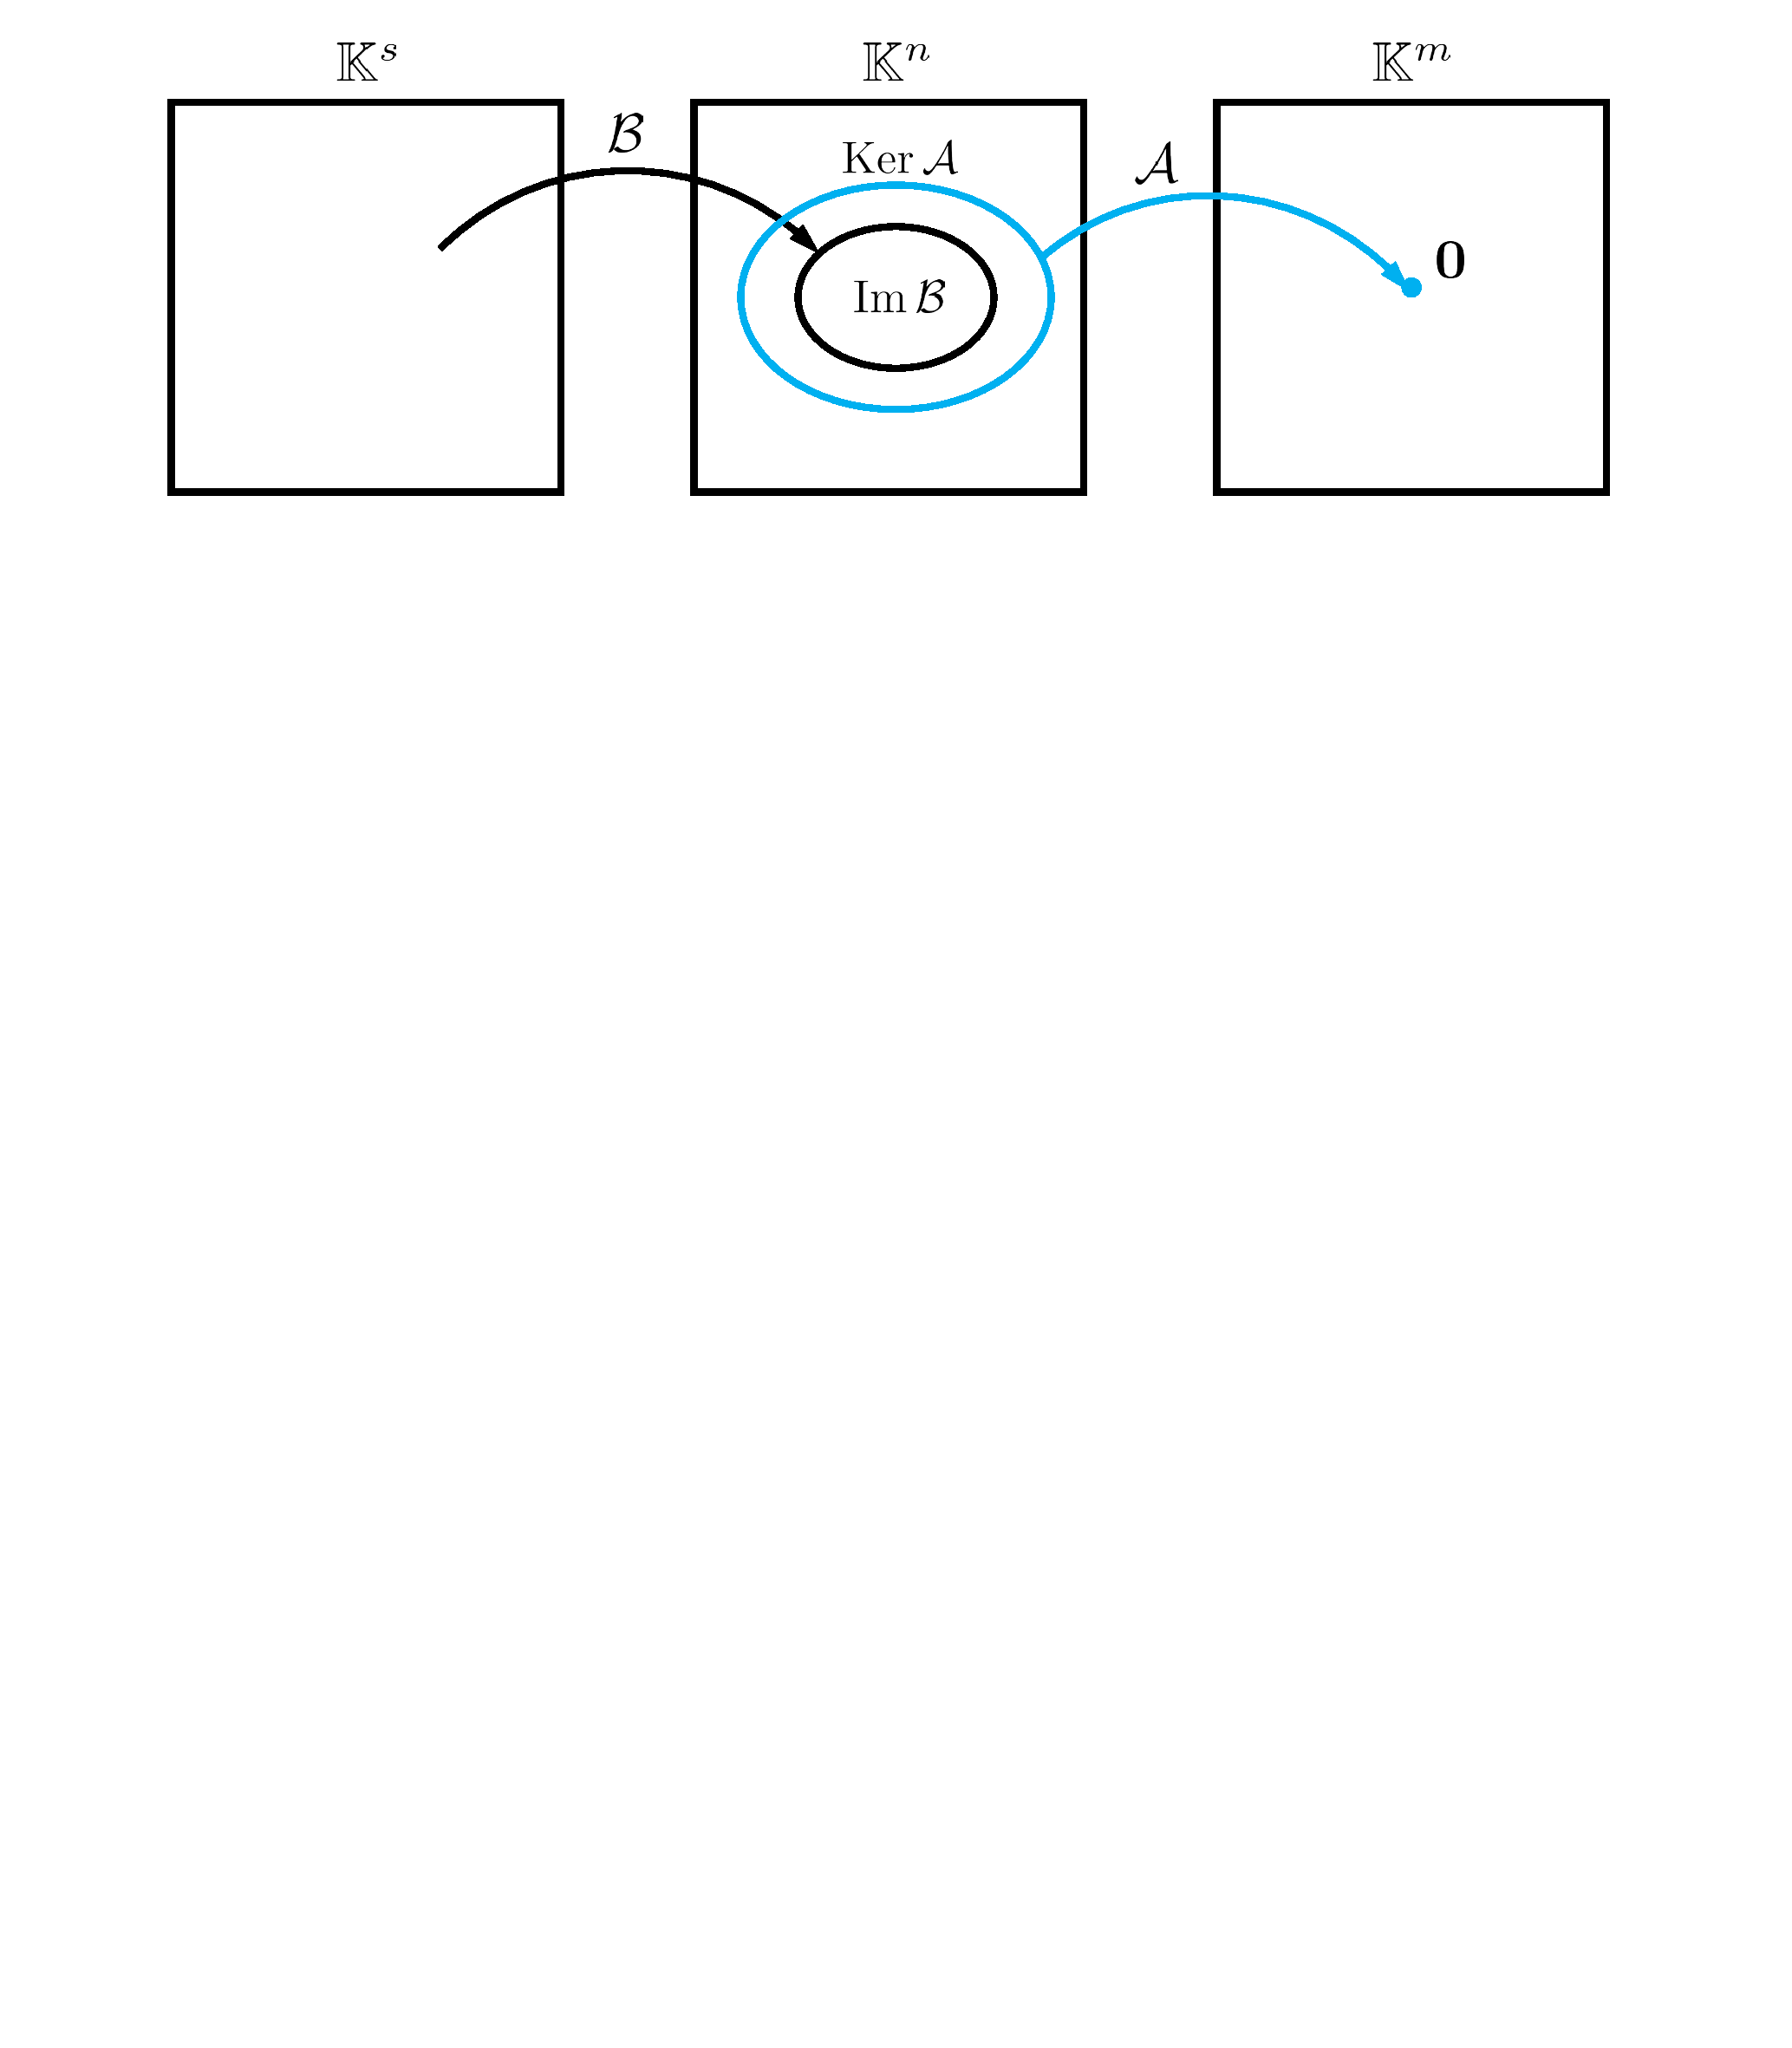
\includegraphics[trim=0 30cm 0 0cm, clip, width=1\textwidth]{fig_AB=O.pdf}
    \caption{例5.8图}
    \label{fig:AB=O}
\end{figure}

\bigskip

\begin{example}
    （例5.3）
    设$A$是$m \times n$矩阵，
    $B$是$n \times r$矩阵，
    $C$是$r \times s$矩阵.

    (1)~~证明Sylvester秩不等式：
    \[
        \mathrm{rank}(A) + \mathrm{rank}(B) - n \le \mathrm{rank}(AB) \\[12pt]
    \]

    (2)~~证明Frobenius秩不等式：
    \[
        \mathrm{rank}(AB) + \mathrm{rank}(BC) - \mathrm{rank}(B) \le \mathrm{rank}(ABC)\\[12pt]
    \]
\end{example}

\begin{proof}
    ~

    (1)~设矩阵$A$表示线性映射$\mathcal{A}: \mathbb{K}^n \to \mathbb{K}^m$，
    矩阵$B$表示线性映射$\mathcal{B}: \mathbb{K}^s \to \mathbb{K}^n$.
    考察复合映射$\mathcal{A} \circ \mathcal{B}$的结构.
    设$\mathcal{A}$在$\operatorname{Im}\mathcal{B}$上的限制为$\mathcal{A}|_{\operatorname{Im}\mathcal{B}}$.
    则$\mathcal{A} \circ \mathcal{B}$与$\mathcal{A}|_{\operatorname{Im}\mathcal{B}} \circ \mathcal{B}$是等同的
    （图\ref{fig:sylv}）.

    列出映射$\mathcal{A}|_{\operatorname{Im}\mathcal{B}}$的维数公式：
    \[
    \dim \operatorname{Im} \mathcal{B}
    = \dim \operatorname{Ker} (\mathcal{A}|_{\operatorname{Im}\mathcal{B}})
    + \dim \operatorname{Im} (\mathcal{A}|_{\operatorname{Im}\mathcal{B}})
    \]
    即：
    \[
    \mathrm{rank}(B)
    = \dim \operatorname{Ker} (\mathcal{A}|_{\operatorname{Im}\mathcal{B}})
    + \mathrm{rank}(AB)~~~~~~(*)
    \]

    将该式对照待证的不等式，
    发现我们只需要搞清楚
    $\dim \operatorname{Ker} (\mathcal{A}|_{\operatorname{Im}\mathcal{B}})$与$n - \mathrm{rank}(A)$的关系.
    再对$\mathcal{A}$列维数公式可知，
    $n - \mathrm{rank}(A) = n - \dim \operatorname{Im} \mathcal{A} = \dim \operatorname{Ker}A$.
    因此我们只要比较$\dim \operatorname{Ker} (\mathcal{A}|_{\operatorname{Im}\mathcal{B}})$与$\dim \operatorname{Ker} \mathcal{A}$的大小.
    
    注意$\mathcal{A}|_{\operatorname{Im}\mathcal{B}}$相比于$\mathcal{A}$缩小了定义域，
    因此$\operatorname{Ker} (\mathcal{A}|_{\operatorname{Im}\mathcal{B}}) \subset \operatorname{Ker} \mathcal{A}$.
    从而$\dim \operatorname{Ker} (\mathcal{A}|_{\operatorname{Im}\mathcal{B}}) \leq \operatorname{Ker} \mathcal{A} = n - \mathrm{rank}(A)$.
    代入$(*)$式，
    就得到了待证的不等式.


    \begin{figure}[H] 
    \centering
    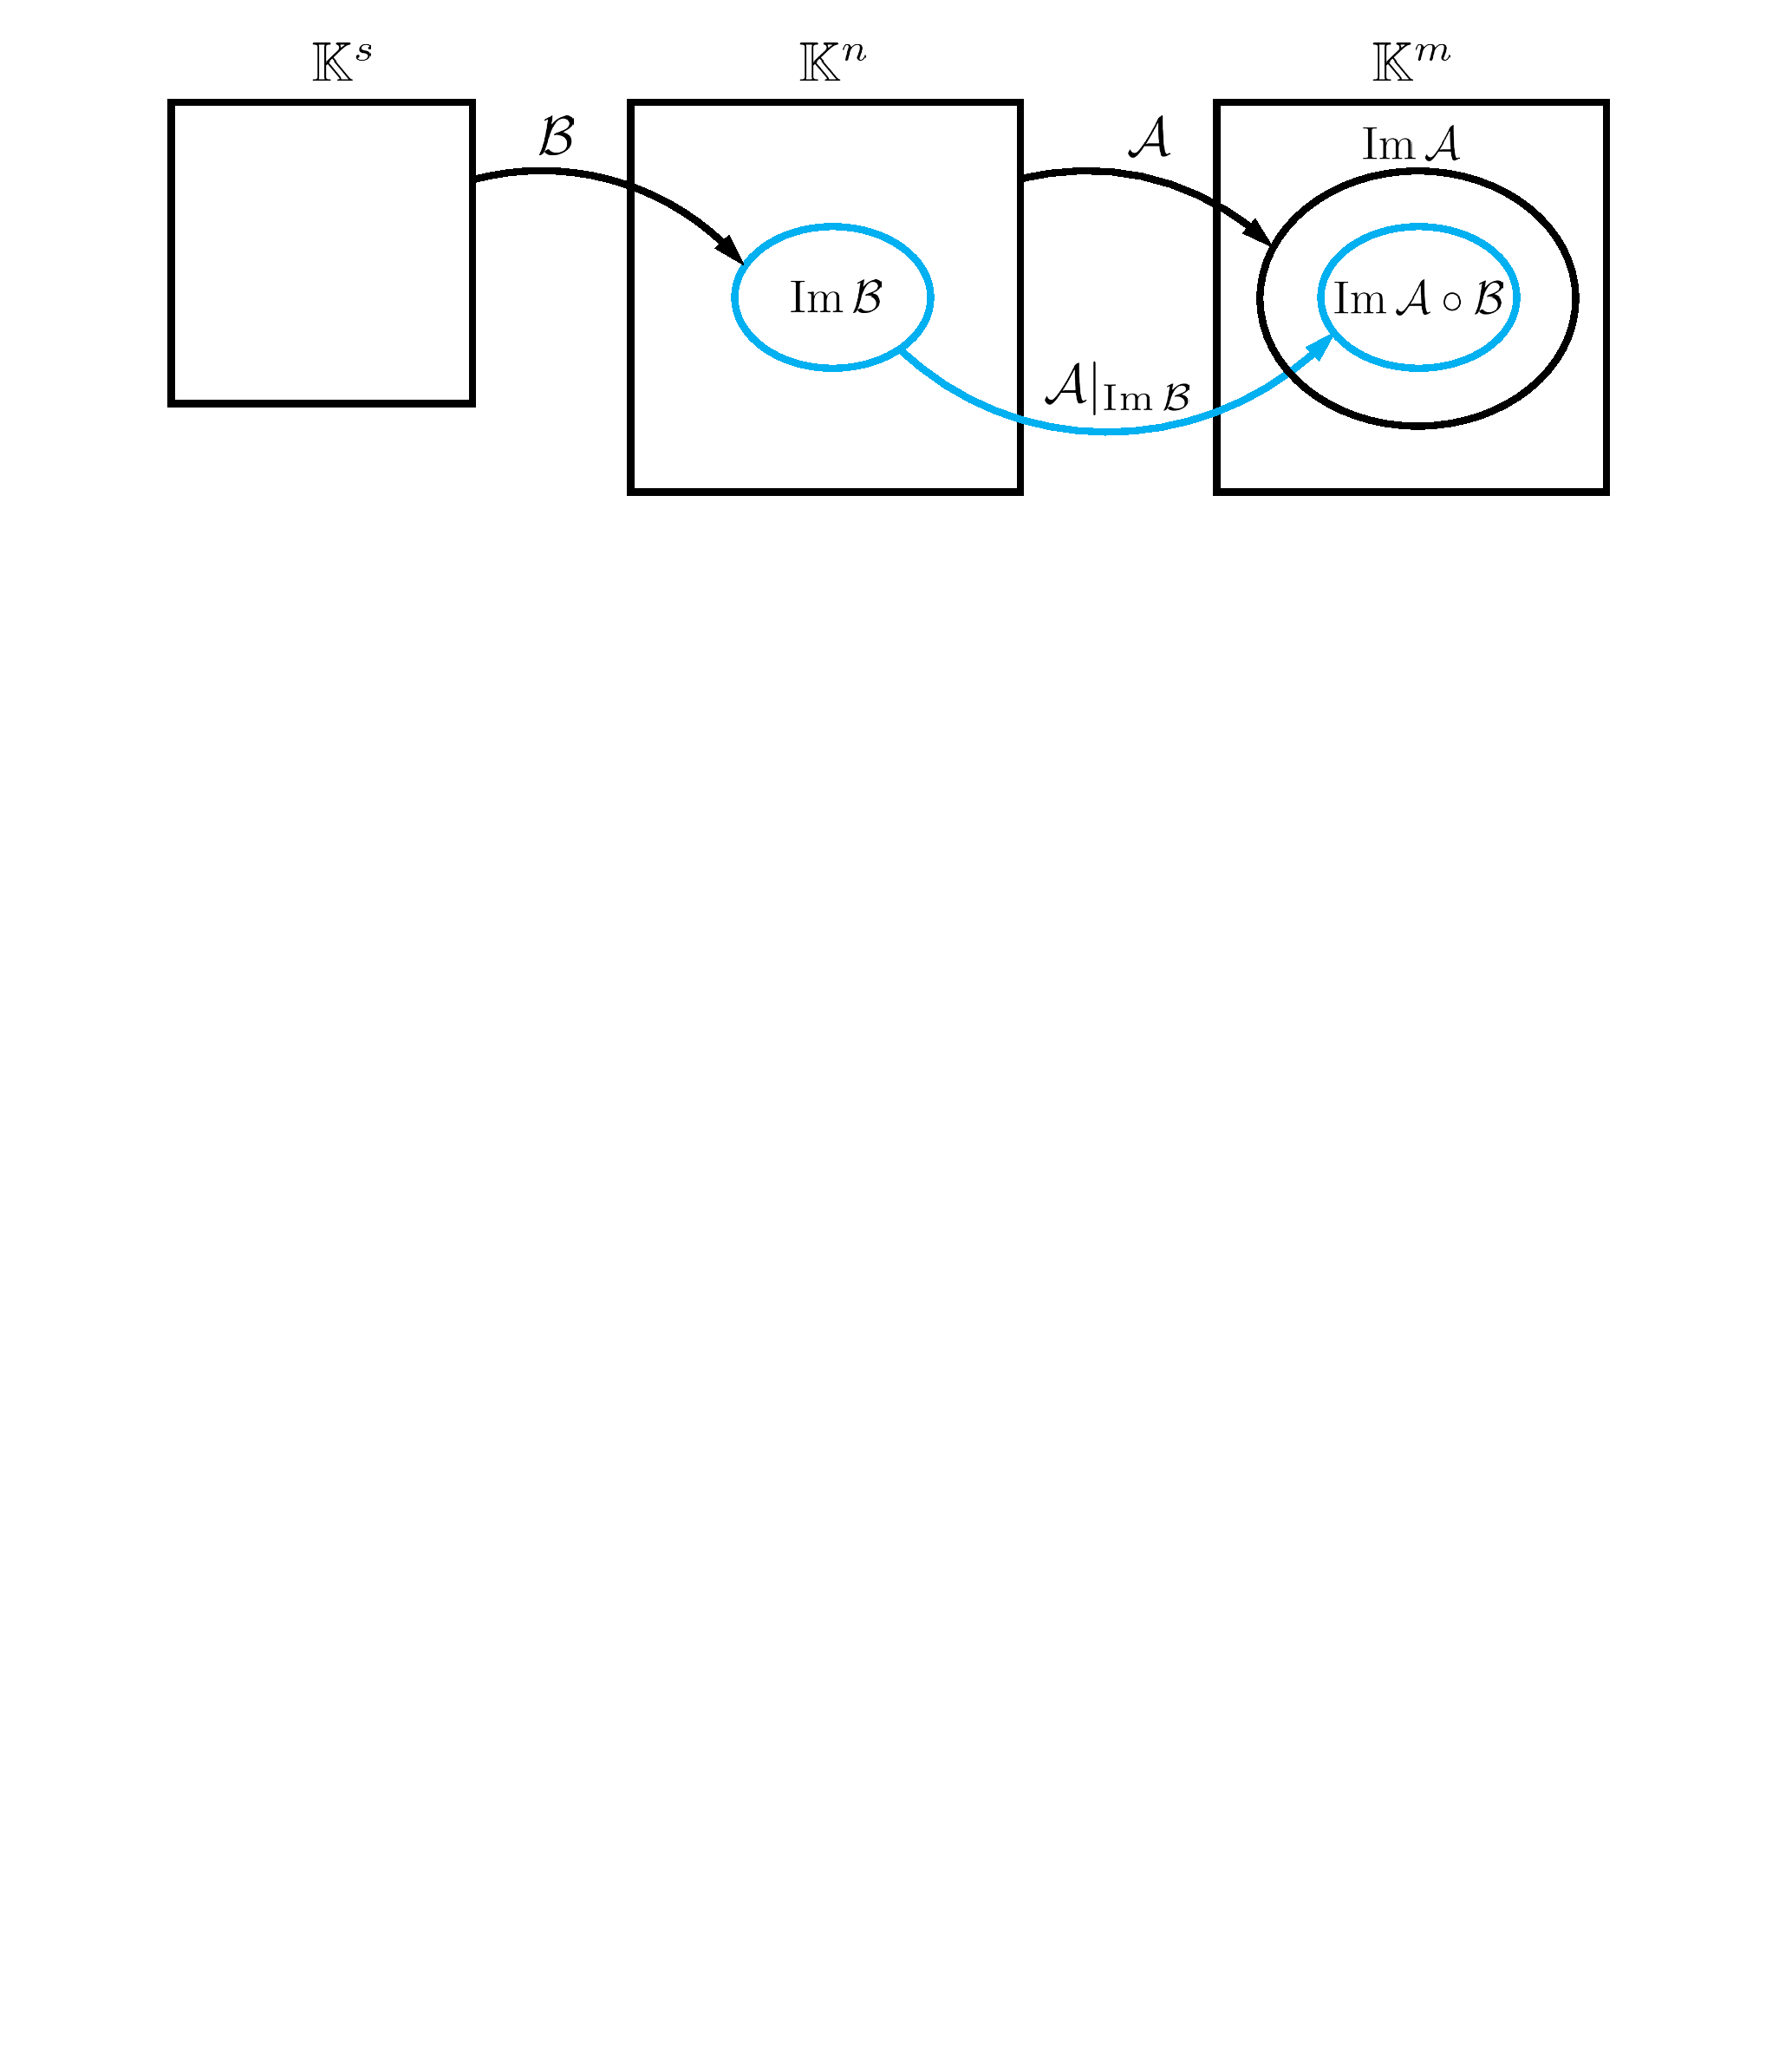
\includegraphics[trim=0 30cm 0 0cm, clip, width=1\textwidth]{fig_sylv.pdf}
    \caption{例5.9(1)图}
    \label{fig:sylv}
    \end{figure}

    \medskip

    (2)~与(1)没有实质的不同，
    只是映射变了，
    映射之间的关系没变，
    参考图\ref{fig:frob}.
    这里设矩阵$C$表示线性映射$\mathcal{C}: \mathbb{K}^r \to \mathbb{K}^s$.
    
    
    列出映射$\mathcal{A}|_{\operatorname{Im}\mathcal{B} \circ \mathcal{C}}$的维数公式：
    \[
    \dim \operatorname{Im} (\mathcal{B} \circ \mathcal{C})
    = \dim \operatorname{Ker} (\mathcal{A}|_{\operatorname{Im}\mathcal{B}\circ \mathcal{C}})
    + \dim \operatorname{Im} (\mathcal{A}|_{\operatorname{Im}\mathcal{B}\circ \mathcal{C}})
    \]
    即：
    \[
    \mathrm{rank}(BC)
    = \dim \operatorname{Ker} (\mathcal{A}|_{\operatorname{Im}\mathcal{B}\circ \mathcal{C}})
    + \mathrm{rank}(ABC)~~~~~~(*)
    \]

    将该式对照待证的不等式，
    发现我们只需要搞清楚
    $\dim \operatorname{Ker} (\mathcal{A}|_{\operatorname{Im}\mathcal{B}\circ \mathcal{C}})$与$\mathrm{rank}(B) - \mathrm{rank}(AB)$的关系.
    再对$\mathcal{A}|_{\operatorname{Im}\mathcal{B}}$列维数公式可知，
    $\mathrm{rank}(B) - \mathrm{rank}(AB) = \dim \operatorname{Im} \mathcal{B} 
    - \dim \operatorname{Im} \mathcal{A}|_{\operatorname{Im}\mathcal{B}} 
    = \dim \operatorname{Ker} \mathcal{A}|_{\operatorname{Im} \mathcal{B}}$.
    因此我们只要比较$\dim \operatorname{Ker} (\mathcal{A}|_{\operatorname{Im}\mathcal{B} \circ \mathcal{C}})$与$\dim \operatorname{Ker} \mathcal{A}|_{\operatorname{Im} \mathcal{B}}$的大小.
    

    注意$\operatorname{Im} \mathcal{B} \circ \mathcal{C} \subset \operatorname{Im} \mathcal{B}$，
    因此$\operatorname{Ker} (\mathcal{A}|_{\operatorname{Im}\mathcal{B} \circ \mathcal{C}}) \subset \operatorname{Ker} (\mathcal{A}|_{\operatorname{Im}\mathcal{B}})$.
    从而$\dim \operatorname{Ker} (\mathcal{A}|_{\operatorname{Im}\mathcal{B} \circ \mathcal{C}}) \leq \dim \operatorname{Ker} (\mathcal{A}|_{\operatorname{Im}\mathcal{B}}) = \mathrm{rank}(B) - \mathrm{rank}(AB)$.
    代入$(*)$式，
    就得到了待证的不等式.


    \begin{figure}[H] 
    \centering
    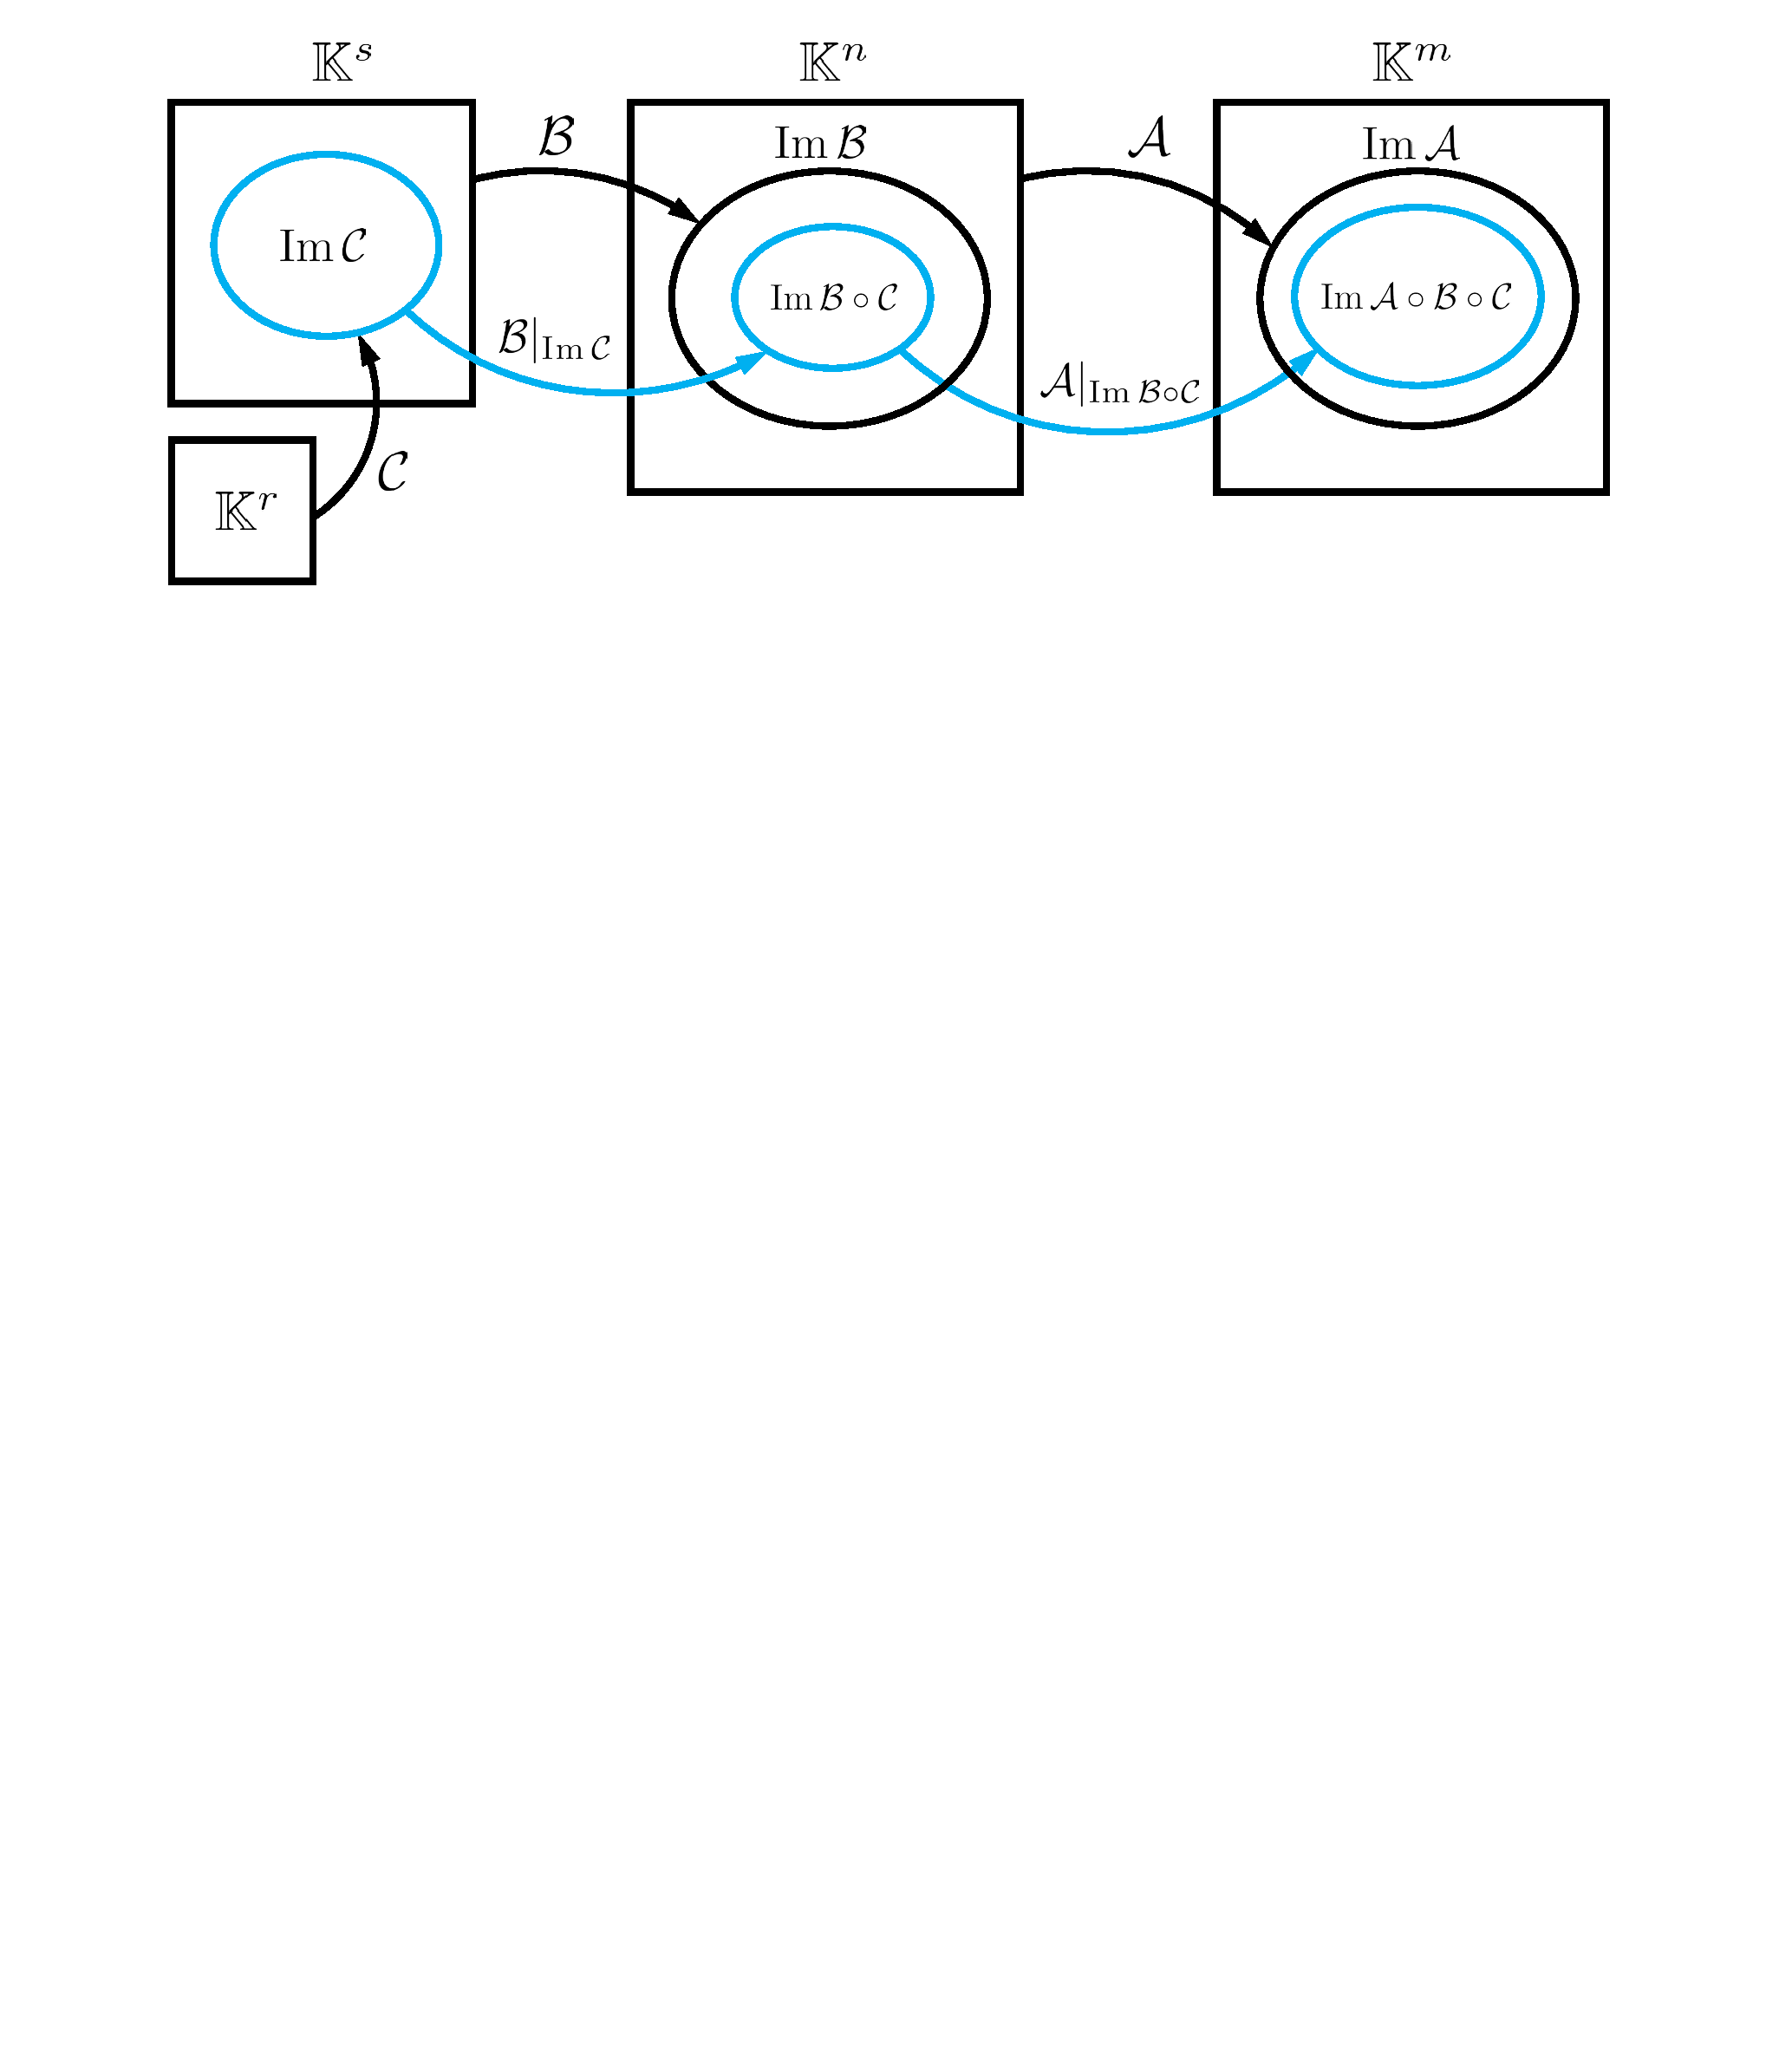
\includegraphics[trim=0 28cm 0 0cm, clip, width=1\textwidth]{fig_frob.pdf}
    \caption{例5.9(2)图}
    \label{fig:frob}
    \end{figure}
\end{proof}


\bigskip


\begin{example}（例5.4）
    ~

    (1)~~求证：$n$阶方阵$A$是幂等矩阵（$A^2 = A$）的充要条件是$\mathrm{rank}(A) + \mathrm{rank}(I_n - A) = n$.

    (2)~~求证：$n$阶方阵$A$是对合矩阵（$A^2 = I_n$）的充要条件是$\mathrm{rank}(I_n + A) + \mathrm{rank}(I_n - A) = n$.
\end{example}

\begin{proof}
    ~

    (1)~“$\Longrightarrow$”：
    若$A^2 = A$，
    则$A(I_n - A) = O$.
    根据例$5.8$的结论，
    $\mathrm{rank}(A) + \mathrm{rank}(I_n - A) \leq n$.
    再根据讲义前文提及的秩不等式，
    $\mathrm{rank}(A) + \mathrm{rank}(I_n - A) \geq \mathrm{rank}(A + I_n - A) = n$.
    二者结合得到$\mathrm{rank} (A)  + \mathrm{rank} (I_n - A)  = n$.

    \smallskip

    “$\Longleftarrow$”：
    若$\mathrm{rank}(A) + \mathrm{rank}(I_n - A) = n$.
    记矩阵$A$表示线性变换$\mathcal{A}: \mathbb{K}^n \to \mathbb{K}^n$，
    恒等映射记为$\mathcal{I}$.
    则$\dim \operatorname{Im} \mathcal{A} + \dim \operatorname{Im} (\mathcal{I} - \mathcal{A}) = n$.
    根据维数公式，
    这等价于$\dim \operatorname{Ker} \mathcal{A} + \dim \operatorname{Ker} (\mathcal{I} - \mathcal{A}) = n$.

    之所以这样考虑，
    是想要借助线性子空间求和的维数公式.
    注意到若非零向量$\bm{x} \in \operatorname{Ker}\mathcal{A}$，
    则它必然不属于$\operatorname{Ker}(\mathcal{I} - \mathcal{A})$.
    这是因为当$\mathcal{A} \bm{x} = \bm{0}$时，
    $(\mathcal{I} - \mathcal{A})\bm{x} = \bm{x}$.
    同理，
    非零向量$\bm{x} \in \operatorname{Ker} (\mathcal{I} - \mathcal{A}) $，
    则$\bm{x} \notin \operatorname{Ker}\mathcal{A}$.
    因此$\operatorname{Ker} \mathcal{A} \cap \operatorname{Ker}  (\mathcal{I} - \mathcal{A}) = \{ \bm{0} \}$.
    此时$\operatorname{Ker} \mathcal{A} + \operatorname{Ker}  (\mathcal{I} - \mathcal{A})$是直和，
    且$\dim (\operatorname{Ker} \mathcal{A} \oplus \operatorname{Ker}  (\mathcal{I} - \mathcal{A})) = \dim \operatorname{Ker} \mathcal{A} + \dim \operatorname{Ker} (\mathcal{I} - \mathcal{A}) = n$
    表明$\operatorname{Ker} \mathcal{A} \oplus \operatorname{Ker}  (\mathcal{I} - \mathcal{A})$是$\mathbb{K}^n$的直和分解.
    因此，任取列向量$\bm{x} \in \mathbb{K}^n$，
    存在唯一分解$\bm{x} = \bm{x}_1 + \bm{x}_2$，
    使得$A\bm{x}_1 = \bm{0}$，$(I_n - A)\bm{x}_2 = \bm{0}$.
    则$A(I_n - A)\bm{x} = (I_n - A)A\bm{x}_1 + A(I_n - A) \bm{x}_2 = \bm{0}$.
    由$\bm{x}$的任意性可知$A(I_n - A) = O$.


    \medskip


    (2)~模仿(1)的证明.
    证明“$\Longleftarrow$”时，
    去证$\mathbb{K}^n = \operatorname{Ker} (\mathcal{I} + \mathcal{A}) \oplus \operatorname{Ker} (\mathcal{I} - \mathcal{A})$.
\end{proof}


\bigskip

\begin{example}（例5.5）
    设$A$为$m \times n$矩阵.
    证明：
    \[
    \mathrm{rank}(I_m - AA^T) - \mathrm{rank}(I_n - A^T A) = m -n
    \]
\end{example}

\begin{proof}
    方便起见，
    记$I_m - AA^T = M$，
    $I_n - A^TA = N$，
    不区分矩阵与线性映射的记号.
    $A$和$A^T$分别是$\mathbb{K}^n \to \mathbb{K}^m$和$\mathbb{K}^m \to \mathbb{K}^n$的线性映射.
    分析待证的式子，
    可用维数公式简化为$\dim \operatorname{Ker}M = \dim \operatorname{Ker}N$.
    为此我们来分析$\operatorname{Ker}M$与$\operatorname{Ker}N$的关系.

    所谓$\operatorname{Ker}M$，
    是指所有满足$(I_m - AA^T) \bm{x} = \bm{0}$的向量$\bm{x} \in \mathbb{K}^m$组成的集合.
    该式等同于$AA^T \bm{x} = \bm{x}$.
    考虑到题中$AA^T$与$A^TA$的对称性，
    将该式两侧左乘$A^T$，
    得到$(A^T A)(A^T \bm{x}) = A^T \bm{x}$，
    即$(I_n  -  A^TA )(A^T \bm{x}) =  N (A^T \bm{x}) = \bm{0}$.
    可见，
    若$\bm{x} \in \operatorname{Ker}M$，
    则$A^T\bm{x} \in \operatorname{Ker}N$.
    换句话说，
    线性映射$A^T$在$\operatorname{Ker}M$上的限制$A^T|_{\operatorname{Ker}M}$
    是$\operatorname{Ker}M \to \operatorname{Ker}N$的映射.

    类似地，
    可以证明$A$在$\operatorname{Ker}N$上的限制$A|_{\operatorname{Ker}N}$
    是$\operatorname{Ker}N \to \operatorname{Ker}M$的映射.

    这里再次强调，上述结论意味着，
    任取$\bm{x} \in \operatorname{Ker}M$，
    有$(AA^T)\bm{x} = \bm{x}$；
    而任取$\bm{y} \in \operatorname{Ker}N$，
    有$(A^T A)\bm{y} = \bm{y}$.
    这说明$A^T|_{\operatorname{Ker}M}$与$A|_{\operatorname{Ker}N}$互为逆映射.
    因此它们都是$\operatorname{Ker}M$与$\operatorname{Ker}N$之间的同构映射.
    而$\operatorname{Ker}M$与$\operatorname{Ker}N$同构就说明$\dim \operatorname{Ker}M = \dim \operatorname{Ker}N$.
\end{proof}

在上一题中，
需要通过巧妙地利用$AA^T$和$A^TA$的对称关系来研究$\operatorname{Ker}M$和$\operatorname{Ker}N$的关系，
并不容易想到.
相比之下，
例5.11所讲的分块矩阵法，
在此题中构造目标是很明确的，
相对比较容易想到.
接下来给出一个分块矩阵构造不容易想到，
而用线性映射很方便的例子.

\bigskip

\begin{example}（例5.6）
    设$A,B$是$n$阶方阵，
    $AB=BA$，
    证明：$\mathrm{rank}(A+B) \leq \mathrm{rank} (A) + \mathrm{rank}(B) - \mathrm{rank}(AB)$.
\end{example}

\begin{remark}
    本题的关键在于正确翻译$AB=BA$这个条件.
\end{remark}

\begin{proof}
    设矩阵$A,B$分别表示$\mathbb{K}^n$上的线性变换$\mathcal{A} , \mathcal{B}$.
    我们知道$\operatorname{Im}(\mathcal{A} \circ \mathcal{B}) = \operatorname{Im}(\mathcal{A}|_{\operatorname{Im}\mathcal{B}}) \subset \operatorname{Im}\mathcal{A}$.
    同理，
    $\operatorname{Im}(\mathcal{B} \circ \mathcal{A}) \subset \operatorname{Im}\mathcal{B}$.
    现在$\mathcal{A} \circ \mathcal{B} = \mathcal{B} \circ \mathcal{A}$，
    于是$ \operatorname{Im}(\mathcal{A} \circ \mathcal{B}) \subset \operatorname{Im}\mathcal{A} \cap \operatorname{Im}\mathcal{B}$，
    因此：

    \[
    \dim \operatorname{Im}(\mathcal{A} \circ \mathcal{B}) \leq \dim \operatorname{Im}\mathcal{A} \cap \operatorname{Im}\mathcal{B}
    \]

    现在涉及两个子空间的交集，
    待证的不等式中又有两个子空间的维数之和，
    想到用维数公式：

    \[
    \dim (\operatorname{Im}\mathcal{A} + \operatorname{Im}\mathcal{B})
    = \dim \operatorname{Im} \mathcal{A} 
    + \dim \operatorname{Im} \mathcal{B}
    - \dim (\operatorname{Im} \mathcal{A} \cap \operatorname{Im} \mathcal{B}  )
    \]

    代入上面的不等式，并代入“秩即像空间维数”的关系，
    得到：
    \[
     \dim (\operatorname{Im}\mathcal{A} + \operatorname{Im}\mathcal{B})
     \leq \mathrm{rank}(A) + \mathrm{rank}(B) - \mathrm{rank}(AB) 
    \]

    对照待证的不等式，
    我们只需要证明$\mathrm{rank}(A+B) = \dim \operatorname{Im}(\mathcal{A}+ \mathcal{B}) \leq \dim (\operatorname{Im}\mathcal{A} + \operatorname{Im}\mathcal{B})$即可.
    任取$\bm{x} \in \mathbb{K}^n$，
    $(\mathcal{A}+\mathcal{B})\bm{x} = \mathcal{A}\bm{x} + \mathcal{B}\bm{x} \in \operatorname{Im}\mathcal{A} + \operatorname{Im}\mathcal{B}$，
    因此$\operatorname{Im}(\mathcal{A}+\mathcal{B}) \subset \dim (\operatorname{Im}\mathcal{A} + \operatorname{Im}\mathcal{B})$，
    从而$\dim \operatorname{Im}(\mathcal{A}+ \mathcal{B}) \leq \dim (\operatorname{Im}\mathcal{A} + \operatorname{Im}\mathcal{B})$成立.
\end{proof}

本题最后证明了不等式$\dim \operatorname{Im}(\mathcal{A}+ \mathcal{B}) \leq \dim (\operatorname{Im}\mathcal{A} + \operatorname{Im}\mathcal{B})$.
而$\dim (\operatorname{Im}\mathcal{A} + \operatorname{Im}\mathcal{B})$正是分块矩阵$(A ~|~B)$的秩.
用该式替换掉待证的不等式之后，
如果再考虑使用分块矩阵法，
则能想到如下的构造思路：

\[
\begin{pmatrix}
    * & * & AB \\
    A & B & O
\end{pmatrix}
\xlongleftarrow{\text{初等变换}}
\begin{pmatrix}
    A & O & O \\
    O & B & O 
\end{pmatrix} \\[12pt]
\]

直接凭空想到这个构造是比较困难的.
而从$AB=BA$的条件入手，
联系到像空间交集和维数公式的运用，
这个思路则比较自然.

\clearpage

\subsubsection{特殊矩阵的性质分析}

本小节的题目涉及一些形式比较特殊的矩阵.
我们先通过下面这道题目摸一摸门道.

\medskip

\begin{example}
    设$A_{n \times n}$是对角线全为$0$的上三角矩阵.
    证明：$A^n = O$.
\end{example}

\begin{remark}
    一个比较寻常的思路是尝试去计算$A^2, A^3, \cdots$，
    发现随着幂次的升高，
    矩阵$0$元素与非零元素的“界限”不断抬高.
    只需要通过直接计算描述出这个规律.

    如果把矩阵当作线性映射看待，
    能提供一个不同的思路.
    我们要计算$A^n$，
    也就是要考察线性变换$A$对任意向量$\bm{x}$连续作用$n$次结果将会如何.
    为此，只需要考察$A$对标准正交基的作用.
\end{remark}

\begin{proof}
    （方法1：直接计算）
    
    设$M_{n \times n}$的$(i,j)$元是$m_{ij}$.
    我们证明一个结论：
    如果矩阵$M$的一条反斜线$j-i = k~(0 \leq k \leq n-1)$及其下方部分的元素全为$0$，
    则$AM$的反斜线$j-i = k+1$及其下方部分的元素全为$0$.
    即：$M$乘$A$之后，分割零元素与非零元素的反斜线会“升高一格”.

    设矩阵$AM$的$(i,j)$元为$b_{ij}$，
    按照矩阵乘法的规则有：
    \[
    b_{ij} = \sum_{p = 1} ^n a_{ip} m_{pj} 
    \]

    考察求和式中的各项何时非零.
    由$A$的定义，
    当$p-i \leq 0$时，
    $a_{ip} = 0$.
    由$M$的定义，
    当$j-p \leq k$时，
    $m_{pj} = 0$.
    因此，
    如果$a_{ip} m_{pj} \ne 0$，
    只可能是$p-i > 0$和$j-p > k$同时满足.
    两式相加，
    可知必须要$j-i > k$.
    因此，当$j-i \leq k+1$时，
    无论$p$取$1$到$n$的何值，
    都有$a_{ip} m_{pj} \ne 0$.
    此时$b_{ij} = 0$.
    根据此结论，
    $A^k$中满足$j-i \leq k-1$的元素皆为$0$.
    对于$k=n$，
    即是说$A^n$满足$j-i \leq n-1$的元素皆为$0$，
    但这是任何指标$(i,j)$都满足的.
    因此$A^n$是零矩阵.
\end{proof}

\begin{proof}
    （方法2：线性变换）

    设$\bm{e}_{j}$是$\mathbb{K}^n$的第$j$个标准正交基，
    即第$j$分量是$1$，其余分量为$0$的向量.
    $A$在$\bm{e}_j$上作用的结果$A \bm{e}_j$正是$A$的第$j$个列向量$\bm{\alpha}_j$.
    根据$A$的定义，
    $\bm{\alpha}_j$的第$j$个分量及之后的分量全为$0$.
    换句话说，
    $A \bm{e}_j = \bm{\alpha}_j \in \langle \bm{e}_1 , \cdots , \bm{e}_{j-1}\rangle$.
    对任意的$\bm{x} = x_1 \bm{e}_1 + x_2 \bm{e}_2 + \cdots + x_r \bm{e}_r \in \langle \bm{e}_1 , \cdots , \bm{e}_r \rangle$，
    有：

    \[
    A \bm{x} 
    = A (x_1 \bm{e}_1 + x_2 \bm{e}_2 + \cdots + x_r \bm{e}_r)
    \in \langle \bm{e}_1 , \cdots , \bm{e}_{r-1}\rangle
    \]

    可见将$A$限制在定义域$\langle \bm{e}_1 , \cdots , \bm{e}_{r} \rangle$上时，
    像空间是$\langle \bm{e}_1 , \cdots , \bm{e}_{r-1} \rangle$
    （直观地说，$A$的作用是从定义域中丢掉角标最大的基向量，从而把空间压缩一个维度）.
    因此，$A$对整个$\mathbb{K}^n = \langle \bm{e}_1 , \cdots , \bm{e}_{n} \rangle$作用$n$次之后（即压缩$n$个维度之后），
    得到平凡子空间$\{ \bm{0} \}$.
    即对任意的$\bm{x} \in \mathbb{K}^n$，
    有$A^n \bm{x} = \bm{0}$.
    这样的$A^n$只能是零矩阵.
\end{proof}

\bigskip

在本题中，
$A$是个很有特点的矩阵，
我们要利用它的特点去解决问题.
第一种方法的思路是直接计算矩阵乘法，
将$A$的特点转化为代数运算中的规律性.
而第二种方法则是先追问
“$A$的这种特殊性意味着什么”.
求助于矩阵的本质（即线性变换）进行探索，
发现所谓“对角线全为$0$的上三角矩阵”
表示的是一种可以不断压缩空间维数的线性变换.
发现这一点之后，
要证的结论就很显然了.



\bigskip

\begin{example}
    设$n$阶方阵$A$的每一行和每一列都只有一个元素是$1$，
    其余元素都是$0$（这种矩阵称为置换矩阵）.
    证明：存在正整数$m$，
    使得$A^m = I$.
\end{example}

\begin{proof}
    设$\bm{e}_{j}$是$\mathbb{K}^n$的第$j$个标准正交基，
    即第$j$分量是$1$，其余分量为$0$的向量.
    按照置换矩阵的定义，
    $A$的列向量组$\bm{\alpha}_1 , \cdots , \bm{\alpha}_n$其实就是一组标准正交基，
    只不过重排了顺序.
    依次记$\bm{\alpha}_1 , \cdots , \bm{\alpha}_n$为$\bm{e}_{i_1}, \bm{e}_{i_2}, \cdots , \bm{e}_{i_n}$，
    其中$i_1 i_2 \cdots i_n$是$1$到$n$某一个排列.
    $A \bm{e}_{j} = \bm{e}_{i_j}$这一事实意味着
    $A$在一组标准正交基上的作用仅仅是重排了它们的顺序.
    $A^m$在一组标准正交基上的作用就是重排了$n$次，
    则$A^m$必定也是置换矩阵.
    但是$1$到$n$的排列方式是有限的（共$n!$种），
    根据抽屉原理，
    如果对标准正交基进行$n!+1$次重排，
    在$n!+1$种排列中必定存在两个相同的排列，
    即$A^1 , A^2 , \cdots , A^{n!}, A^{n!+1}$中必有两个相同的.
    不妨设$A^{r} = A^{r+m}$，
    则$A^m$就是单位矩阵.
\end{proof}

\bigskip

\begin{example}
    设$a,b,c,d$是非零实数，
    求下列矩阵的逆：
    \[
    A = 
    \begin{pmatrix}
        a & b & c & d \\
        -b & a & -d & c \\
        -c & d & a & -b \\
        -d & -c & b & a 
    \end{pmatrix}
    \]
\end{example}

\begin{remark}
    本题的矩阵有一定对称性，
    “看法”是不唯一的.
    方法1的“看法”是注意到$A$是正交矩阵.
    方法2的“看法”是利用上一题中的置换矩阵.
\end{remark}

\begin{proof}
    （方法1）

    观察矩阵的列向量组$\bm{\alpha}_1 , \cdots , \bm{\alpha}_4$，
    发现它们两两正交，
    即满足$\bm{\alpha}_i ^T \bm{\alpha}_j = 0$.
    从这个表达式就可以看出$A^T A$是对角矩阵.
    通过计算发现$A^T A = (a^2 + b^2 + c^2 + d^2)I$.
    则$A^{-1} = \frac{1}{a^2 + b^2 + c^2 + d^2} A^T$.

\end{proof}

\begin{proof}
    （方法2）

    将矩阵元素排列的规律用置换矩阵来描述.
    分别按照$a,b,c,d$去定义以下$4$个置换矩阵：
    \[
    E_1 = I,~
    E_2 = 
    \begin{pmatrix}
        0 & 1 & 0 & 0 \\
        -1 & 0 & 0 & 0 \\
        0 & 0 & 0 & -1 \\
        0 & 0 & 1 & 0
    \end{pmatrix},~
    E_3 = 
    \begin{pmatrix}
        0 & 0 & 1 & 0 \\
        0 & 0 & 0 & 1 \\
        -1 & 0 & 0 & 0 \\
        0 & -1 & 0 & 0
    \end{pmatrix},~
    E_4 = 
    \begin{pmatrix}
        0 & 0 & 0 & 1 \\
        0 & 0 & -1 & 0 \\
        0 & 1 & 0 & 0 \\
        -1 & 0 & 0 & 0
    \end{pmatrix}
    \]

    置换矩阵的乘积依然是置换矩阵，
    我们考察这些置换矩阵之间的代数关系.
    重点关注$E_2, E_3, E_4$.
    通过计算得到以下的乘法表
    【矩阵$A$与四元数$a + bi + cj + dk$有何联系？】：

    \begin{eq1}
        &E_2 \cdot E_2 = E_3 \cdot E_3 = E_4 \cdot E_4 = -E_1 \\[6pt]
        &E_2 \cdot E_3 = -E_3 \cdot E_2 = E_4 \\[6pt]
        &E_3 \cdot E_4 = -E_4 \cdot E_3 = E_2 \\[6pt]
        &E_4 \cdot E_2 = -E_2 \cdot E_4 = E_3 \\[12pt]
    \end{eq1}

    可见$E_1 , E_2 , E_3 , E_4$构成了一个封闭的代数体系.
    $A = a E_1 + b E_2 + c E_3 + d E_4$.
    我们寻找一个同样具有形式$p E_1 + q E_2 + r E_3 + s E_4$的矩阵$B$，
    使得$AB$是数量矩阵$ = \lambda E_1$.
    考察矩阵乘法：

    \[
    (a E_1 + b E_2 + c E_3 + d E_4)(p E_1 + q E_2 + r E_3 + s E_4)
    \]

    在乘法代数展开式中，
    所有的平方项实质都是$E_1$的倍数，
    而所有的交叉项实质都是$E_2, E_3$或$E_4$，
    是我们所不要的.
    因此一个简单的想法是取$p,q,r,s$让所有的交叉项抵消.
    最方便的是让$(p,q,r,s) = (a,-b,-c,-d)$.
    此时有：

    \begin{eq1}
    (a E_1 + b E_2 + c E_3 + d E_4)(a E_1 + -b E_2 + -c E_3 + -d E_4)
    = (a^2 + b^2 + c^2 + d^2) E_1 \\[12pt]
    \end{eq1}

    所以$A^{-1} = \frac{1}{a^2 + b^2 + c^2 + d^2}(a E_1 + -b E_2 + -c E_3 + -d E_4)$.
\end{proof}


~\par

\begin{example}~
    
    (1)~设$A$是$n$阶方阵，满足
    $A^k = O$，
    $k$是正整数.
    证明：$I-A$可逆.

    (2)~设$A$是$n$阶方阵，满足
    $A^2 = A$，
    证明：$A - 2I$可逆.

    (3)~设矩阵：
    \begin{eq1}
        A = 
        \begin{pmatrix}
            -1 & 1 & 1 & 1 & 1 \\[4pt]
            1 & -1 & 1 & 1 & 1 \\[4pt]
            1 & 1 & -1 & 1 & 1 \\[4pt]
            1 & 1 & 1 & -1 & 1 \\[4pt]
            1 & 1 & 1 & 1 & -1
        \end{pmatrix} \\[12pt]
    \end{eq1}

    求$A$的逆.
\end{example}

\begin{remark}
    证明矩阵可逆的一种特殊的方法是，
    通过矩阵的代数计算直接找到逆矩阵.
    第(3)问直接用初等变换法求逆当然是可以的，
    不过参考第(2)问，
    可以开发出一种巧妙的新思路.
\end{remark}

\begin{solution}~

    (1)~
    $I = I-A^k = (I-A)(I + A + A^2 + \cdots + A^{k-1})$
    ，因此$I + A + A^2 + \cdots + A^{k-1}$就是$I-A$的逆矩阵.


    \medskip

    (2)~
    用待定系数法，
    设$A-2I$的逆矩阵形如$pA+qI$，
    即$(A-2I)(pA+qI) = I$.
    计算左侧得到：
    \[
    (A-2I)(pA+qI)
    = pA^2 + (q-2p)A - 2qI
    = (q-p)A - 2qI
    \]
    解得$p = -\frac{1}{2}, ~q = -\frac{1}{2}$.
    因此$A-2I$的逆矩阵是$-\frac{1}{2}A - \frac{1}{2}I$.

    \medskip

    (3)~记$5$阶单位矩阵为$I$，
    元素全为$1$的$5$阶方阵为$J$，
    则$A = J - 2I$.
    通过直接计算可知$J$具有性质$J^2 = 5J$.
    猜测$A = J-2I$的逆矩阵形如$pJ + qI$.
    即$(J - 2I) (pJ + qI) = I$.
    计算左侧得到：
    \[
    (J - 2I) (pJ + qI)
    = pJ^2 + (q - 2p)J - 2qI
    = (q + 3p)J - 2qI
    \]
    解得$p = \frac{1}{6}, ~q = -\frac{1}{2}$，
    因此$J - 2I$的逆矩阵是$\frac{1}{6}J - \frac{1}{2}I$，
    即：
    
    \[
    A^{-1} = 
    \frac{1}{6}
    \begin{pmatrix}
        -2 & 1 & 1 & 1 & 1 \\[4pt]
        1 & -2 & 1 & 1 & 1 \\[4pt]
        1 & 1 & -2 & 1 & 1 \\[4pt]
        1 & 1 & 1 & -2 & 1 \\[4pt]
        1 & 1 & 1 & 1 & -2 
    \end{pmatrix}
    \]

\end{solution}

\bigskip

\subsubsection{伴随矩阵}

\begin{example}
    设$A$是$n$阶方阵.
    $A^*$是$A$是伴随矩阵.

    (1)~~
    证明：

    \begin{eq1}
        \mathrm{rank}(A^*) = 
        \begin{cases}
            n, \quad \mathrm{rank}(A) = n \\[2pt]
            1, \quad \mathrm{rank}(A) = n-1 \\[2pt]
            0, \quad \mathrm{rank}(A) \le n-2 
        \end{cases} \\[12pt]
    \end{eq1}

    (2)~~
    若已知$|A|$，如何计算$|A^{*}|$？
\end{example}

\begin{remark}
    虽然伴随矩阵的一个重要功能是求逆，
    但是讨论伴随矩阵时并不总是默认$A$是可逆的，
    此时求逆公式就用不上了.
    需要知道伴随矩阵的重要性质$AA^* = |A|I_n$.
    这条公式在$A$不可逆时也适用，此时$AA^* = O$.

    第(2)问的易错点在于$|kA|=k^n |A|$，
    注意不要以为$|kA| = k |A|$.
\end{remark}

\begin{solution}

    (1)~
    分三种情况讨论.

    (i)~当$\operatorname{rank}(A)=n$时，
    因此 $A$ 可逆，
    此时有
    $
    A^*=|A|A^{-1}
    $，
    且$|A| \ne 0$.
    所以$\operatorname{rank}(A^*)= \operatorname{rank}(A^{-1}) =n$

    \smallskip

    (ii)~当$\operatorname{rank}(A)=n-1$时，
    $|A|=0$，
    但存在至少一个$A$的$(n-1)$ 阶子式不为零，
    即$A^*$不是零矩阵.
    但由伴随矩阵性质，
    $AA^*=O$，
    于是 $A^*$ 的每一列都属于齐次方程组
    $
    A \bm{x} = \bm{0}
    $
    的解空间.
    根据维数公式，
    解空间的维数为$n - \mathrm{rank}(A) = 1$.
    因此 $A^*$ 的所有列向量都属于同一个一维空间，
    故所有列向量线性相关，并且至少有一列非零.
    因此
    $
    \operatorname{rank}(A^*)=1.
    $

    \smallskip

    (iii)~当$\operatorname{rank}(A)\le n-2$时，
    $A$ 的所有 $(n-1)$ 阶子式全部为零，
    根据伴随矩阵的定义，
    $A^*$是零矩阵，
    故
    $
    \operatorname{rank}(A^*)=0
    $.

    综上：

    \[
    \operatorname{rank}(A^*)=
    \begin{cases}
    n, & \operatorname{rank}(A)=n,\\[4pt]
    1, & \operatorname{rank}(A)=n-1,\\[4pt]
    0, & \operatorname{rank}(A)\le n-2.
    \end{cases}
    \]

   \medskip

   (2)~ 由伴随矩阵性质
    $
    AA^*=|A|I_n.
    $，
    两边取行列式：
    $
    \det (AA^*) = \det ( \det (A) I_n ).
    $
    等号左侧为$|A| \cdot |A^*|$，
    等号右侧为$|A|^n$.

    若 $|A|\neq 0$，则两边除以 $|A|$，
    得到
    $
    |A^*|=(|A|)^{n-1}.
    $

    当 $|A|=0$ ，
    由(1)的结论知
    $
    |A^*|=0.
    $

    上面两种情形下的公式可以统一写成：
    $
    |A^*|=(|A|)^{\,n-1}.
    $
\end{solution}

在有关伴随矩阵的问题中，
例5.18的结论是基础性的.
到目前为止，
矩阵的证明题无非是围绕秩和行列式这些基础概念展开的.
而例5.18就搞清楚了伴随矩阵的秩和行列式.
下面给出两个简单的应用作为示范.

\bigskip

\begin{example}
    设$n (n \geq 2)$阶方阵$A$
    恰有$k$个$n-1$阶子式等于$0$，
    其中$1 \leq k \leq n-1$.
    证明：$|A| \ne 0$.
\end{example}

\begin{proof}
    反证法.
    假设$|A| = 0$.
    则$\mathrm{rank}(A) \leq n-1$.
    由于$k \leq n-1$，
    所以$A^* \ne O$.
    根据例5.18的结论，
    可知$\mathrm{rank}(A^*) = 1$.

    $A$有$k$个$n-1$阶子式，
    即$A^*$中有$k$个元素为$0$.
    $k \leq n-1$
    表明$A^*$的每一行和每一列都不是零向量.
    但是，若选取$A^*$的一个含有$0$的列向量，
    设其第$i$分量为$0$.
    由于$\mathrm{rank}(A^*) = 1$，
    可知$A^*$的所有列向量都是它的倍数，
    因此每个列向量第$i$分量都是$0$，
    从而$A^*$的第$i$行是零向量，
    矛盾.
\end{proof}

\clearpage

\begin{example}
    设$A$是$n(n>2)$阶方阵.
    求$(A^*)^*$.
\end{example}

\begin{solution}
    如果$A$可逆，
    则$A^*$也可逆.
    利用公式$A^* = |A|A^{-1}$，
    有：
    \[
    (A^*)^* = |A^*| (A^*)^{-1}
    = |A|^{n-1} |A|^{-1} A 
    = |A|^{n-2} A
    \]

    如果$A$不可逆，
    即$\mathrm{rank}(A) \leq n-1$，
    则$\mathrm{rank}(A^*) \leq 1$，
    而$\mathrm{rank}(A^*)^* = 0$，
    即$A^* = O$.
\end{solution}

\subsubsection{降阶公式}


\begin{example}
    设$A$是$m$阶方阵，
    $D$是$n$阶方阵，
    $B$是$m \times n$矩阵，
    $C$是$n \times n$矩阵.

    (1)~
    如果$A$可逆，证明：

    \begin{eq1}
        \begin{vmatrix}
            A & B \\[4pt]
            C & D 
        \end{vmatrix}
        = |A||D - CA^{-1}B| \\[12pt]
    \end{eq1} 

    (2)~如果$D$可逆，
    是否能得到类似的结论？
\end{example}

\begin{remark}
    求分块矩阵的行列式，
    根据Laplace展开公式，
    只需要化成分块上三角或者分块下三角.
\end{remark}

\begin{proof}

    (1)~
    \[
    \det 
    \begin{pmatrix}
        A & B \\[4pt]
        C & D
    \end{pmatrix}
    \xlongequal{r_2 + CA^{-1} \cdot r_1}
    \det
    \begin{pmatrix}
        A & B \\[4pt]
        O & D-CA^{-1}B
    \end{pmatrix}
    = \det (A) \cdot \det (D-CA^{-1}B)
    \]

    (2)~
    \[
    \det 
    \begin{pmatrix}
        A & B \\[4pt]
        C & D
    \end{pmatrix}
    \xlongequal{r_1 + BD^{-1} \cdot r_2}
    \det
    \begin{pmatrix}
        A-BD^{-1}C & O \\[4pt]
        C & D
    \end{pmatrix}
    = \det (D) \cdot \det (A-BD^{-1}C)
    \]

\end{proof}

\bigskip

在上一题的设定中，
如果$A,D$都可逆，
结合两个小问的结论，
我们得到一个公式：

\begin{eq1}
    |A| |D - CA^{-1}B|
    = |D| |A-BD^{-1}C|
\end{eq1}

这个公式称为
\textbf{降阶公式}.
之所以“降阶”，
是关注到$m$和$n$可能不同，
也就是等号两侧分别是一些$m$和$n$阶矩阵的行列式.
因此，利用这个公式可以将高阶的行列式化成低阶的行列式.
接下来通过两个例子展示具体做法.

\clearpage


\begin{example}
    
    计算下列矩阵行列式的值：

    \begin{eq1}
        M = 
        \begin{pmatrix}
            a_1^2 & a_1a_2 +1 & \cdots & a_1 a_n + 1 \\[4pt]
            a_2a_1 + 1 & a_2^2 & \cdots & a_2 a_n + 1 \\[4pt]
            \vdots & \vdots & \ddots & \vdots \\[4pt]
            a_na_1+ 1& a_na_2 + 1& \cdots & a_n^2
        \end{pmatrix} \\[12pt]
    \end{eq1}
\end{example}

\begin{remark}
    $M$的特点是关于$a_i a_j$的规律，
    但是对角线的规律相对特殊，
    缺少“$+1$”.
    这是可以用降阶公式的信号.
    诀窍是尝试把$M$看成降阶公式中的
    $A - BD^{-1}C$.
    其中$D$取成单位矩阵，
    而$A$是对角矩阵，
    负责分离出对角线的特征.
    最后按照矩阵整体的规律，
    设法将其分解成$BC$即可.
\end{remark}

\begin{solution}
    
    将$M$化为：
    \[
    M = -I_n + 
    \begin{pmatrix}
    a_1 & 1\\
    a_2 & 1\\
    \vdots & \vdots\\
    a_n & 1
    \end{pmatrix}
    I_2^{-1}
    \begin{pmatrix}
    a_1 & a_2 & \cdots & a_n\\
    1 & 1 & \cdots & 1
    \end{pmatrix}
    \]
    
    由降阶公式得到：
    \begin{eq1}
        |M| &= |I_2|^{-1} |-I_n|
        \left|
        I_2 +
        \begin{pmatrix}
        a_1 & a_2 & \cdots & a_n\\
        1 & 1 & \cdots & 1
        \end{pmatrix}
        (-I_n)^{-1}
        \begin{pmatrix}
        a_1 & 1\\
        a_2 & 1\\
        \vdots & \vdots\\
        a_n & 1
        \end{pmatrix}
        \right|  \\[4pt]
        &= (-1)^n 
        \left|
        I_2 -
        \begin{pmatrix}
        \sum\limits_{i=1}^n a_i^2 & \sum\limits_{i=1}^n a_i\\
        \sum\limits_{i=1}^n a_i & n
        \end{pmatrix}
        \right| \\[4pt]
        &= (-1)^n 
        \left(
        (1 - n)\left(1 - \sum\limits_{i=1}^n a_i^2\right)
        - \left(\sum\limits_{i=1}^n a_i\right)^2
        \right)
    \end{eq1}

\end{solution}

\bigskip

\begin{example}
    计算下列矩阵行列式的值：

    \begin{eq1}
        M =
        \begin{pmatrix}
            0 & 2 & 3 & \cdots & n \\[4pt]
            1 & 0 & 3 & \cdots & n \\[4pt]
            1 & 2 & 0 & \cdots & n \\[4pt]
            \vdots & \vdots & \vdots & \ddots & \vdots \\[4pt]
            1 & 2 & 3 &\cdots & 0
        \end{pmatrix}\\[12pt]
    \end{eq1}
\end{example}

\begin{remark}
    技巧同上.
\end{remark}

\begin{solution}
    
    将$M$化为：
    \[
    M =
    \begin{pmatrix}
        -1 & 0 & \cdots & 0 \\
        0 & -2 & \cdots & 0 \\
        \vdots & \vdots & \ddots & \vdots \\
        0 & 0 & \cdots & -n 
    \end{pmatrix}
    + 
    \begin{pmatrix}
    1 & 0\\
    1 & 0\\
    \vdots & \vdots\\
    1 & 0
    \end{pmatrix}
    I_2^{-1}
    \begin{pmatrix}
    1 & 2 & \cdots & n\\
    0 & 0 & \cdots & 0
    \end{pmatrix}
    \]

    由降阶公式得到$|M|$的值为：

    \begin{eq1}
        &|I_2|^{-1}
        \cdot 
        \det \begin{pmatrix}
        -1 & 0 & \cdots & 0 \\
        0 & -2 & \cdots & 0 \\
        \vdots & \vdots & \ddots & \vdots \\
        0 & 0 & \cdots & -n 
    \end{pmatrix}
    \cdot 
    \det 
    \left(
        I_2 +
    \begin{pmatrix}
        1  & \cdots & n \\
        0  & \cdots & 0 \\
    \end{pmatrix}
    \begin{pmatrix}
        -1 & 0 & \cdots & 0 \\
        0 & -2 & \cdots & 0 \\
        \vdots & \vdots & \ddots & \vdots \\
        0 & 0 & \cdots & -n 
    \end{pmatrix}^{-1}
    \begin{pmatrix}
        1 & 0 \\
        1 & 0 \\
        \vdots & \vdots \\
        1 & 0 & 
    \end{pmatrix}
    \right) \\[8pt]
    &= (-1)^n n!\cdot 
    \det
    \left(
        I_2 + 
    \begin{pmatrix}
        1  & \cdots & n \\
        0  & \cdots & 0 \\
    \end{pmatrix}
    \begin{pmatrix}
        -1 & 0 & \cdots & 0 \\
        0 & -1/2 & \cdots & 0 \\
        \vdots & \vdots & \ddots & \vdots \\
        0 & 0 & \cdots & -1/n 
    \end{pmatrix}
    \begin{pmatrix}
        1 & 0 \\
        1 & 0 \\
        \vdots & \vdots \\
        1 & 0 & 
    \end{pmatrix}
    \right)\\[8pt]
    &= (-1)^n n!\cdot 
    \det
    \left(
        I_2 + 
    \begin{pmatrix}
        1  & \cdots & n \\
        0  & \cdots & 0 \\
    \end{pmatrix}
    \begin{pmatrix}
        -1 & 0 & \cdots & 0 \\
        0 & -1/2 & \cdots & 0 \\
        \vdots & \vdots & \ddots & \vdots \\
        0 & 0 & \cdots & -1/n 
    \end{pmatrix}
    \begin{pmatrix}
        1 & 0 \\
        1 & 0 \\
        \vdots & \vdots \\
        1 & 0 & 
    \end{pmatrix}
    \right) \\[8pt]
    &= (-1)^n n!\cdot 
    \det
    \left(
        \begin{pmatrix}
            1 & 0 \\
            0 & 1
        \end{pmatrix}
        +
        \begin{pmatrix}
            -n & 0 \\
            0 & 0
        \end{pmatrix}
    \right)
    =  (-1)^{n+1} n! (n-1)
    \end{eq1}  
\end{solution}

\bigskip

\subsubsection{摄动法}

\begin{example}
    设$A$是不可逆的$n$阶方阵.
    证明：
    存在$\lambda = 0$的去心邻域，
    使得$A + \lambda I_n$可逆.
\end{example}

\begin{proof}
    $|A + \lambda I_n|$是
    关于$\lambda$的$n$次多项式，
    至多有$n$个零点，
    $\lambda = 0$是其中之一.
    除了$\lambda =0$之外，
    其余$n-1$的零点的绝对值最小者记为$\lambda_0$.
    则当$\lambda$属于半径为$|\lambda_0|$的去心领域$U(0,|
    \lambda_0|)$时，
    $|A + \lambda I_n|\ne 0 $，
    即$A+\lambda I_n$可逆.
\end{proof}

这一题的结论给我们很大的启发：
对于不可逆矩阵$A$，
对其施加一个很小的扰动$\lambda I_n$，
就能使其成为可逆矩阵.
通过这个手法，
我们就可以把不可逆的矩阵当作可逆矩阵来处理.
这种方法称为\textbf{摄动法}.

\begin{example}
    设$A,B,C,D$都是$n$阶实方阵，
    且满足$AC=CA$.
    证明：

    \begin{eq1}
        \begin{vmatrix}
            A & B \\[4pt]
            C & D 
        \end{vmatrix} 
        = 
        |AD-CB| \\[12pt]
    \end{eq1}
\end{example}

\begin{remark}
    本题中没有说$A,B,C,D$可逆，
    阻止了我们做初等行变换.
    使用摄动法就可以绕过这个阻碍.
\end{remark}

\begin{proof}

    如果$A$可逆，
    可以做分块初等变换，推导出降阶公式：
    \[
    \det 
    \begin{pmatrix}
        A & B \\
        C & D
    \end{pmatrix}
    = 
    \det 
    \begin{pmatrix}
        A & B \\
        O & D - CA^{-1}B
    \end{pmatrix}
    = |A| |D - CA^{-1}B|
    \]

    利用$AC=CA$，
    可以进一步得到：
    \[
     \det 
    \begin{pmatrix}
        A & B \\
        C & D
    \end{pmatrix}
    = |AD - ACA^{-1}B|
    = |AD - CAA^{-1}B|
    = |AD-CB|
    \]

    若$A$不可逆，
    使用摄动法.
    存在$0$的一个小去心邻域$U$，
    使得$\lambda = U$时，
    有$A + \lambda I_n$可逆.
    用$A + \lambda I_n$代替$A$，
    有：
    \[
     \det 
    \begin{pmatrix}
        A + \lambda I_n & B \\
        C & D
    \end{pmatrix}
    = |(A + \lambda I_n)D-CB|
    \]

    注意等号两边都是关于$\lambda$的$n$次多项式.
    现在这两个多项式在$\lambda \in U$时处处成立，
    即有无穷多个$\lambda$使得这两个多项式相等，
    意味着它对于$\lambda \in \mathbb{R}$是恒等式，
    因此也对$\lambda = 0$成立.    
\end{proof}

\bigskip

\begin{example}
    设$A,B$是$n$阶矩阵，
    $n \geq 2$.
    证明：$(AB)^* = B^*A^*$.
\end{example}

\begin{proof}
    若$A,B$均可逆，
    则利用公式$A^* = |A|A^{-1}$，
    可得：
    \[
    (AB)^* = |AB|(AB)^{-1} = |B|B{-1} \cdot |A| A^{-1} = B^*A^*
    \]
    
    若$A,B$其中之一不可逆，
    使用摄动法.
    考虑矩阵$A(\lambda) = A + \lambda I_n$，
    $B(\lambda) = B + \lambda I_n$.
    则存在$0$的去心邻域$U$，
    使得$\lambda \in U$时，
    $A(\lambda) , B(\lambda)$均可逆.
    则有：
    \[
    (A(\lambda) B(\lambda))^* = B(\lambda)^* A(\lambda)^*
    \]

    该等式左右两侧的每个矩阵元都是关于$\lambda$的有限阶多项式.
    但是等式对$\lambda \in U$成立，
    即有无穷多个$\lambda$使得等式成立.
    因此该式是关于$\lambda$的恒等式，
    对于$\lambda = 0$也成立，
    即$(AB)^* = B^*A^*$.
\end{proof}

\bigskip


\begin{comment}
    \subsubsection{其他}

    \begin{example}
        ~

        (1)~设 $A,B$ 分别为 $m \times n$ 和 $n\times m$ 矩阵，
        证明：若矩阵 $I_n + AB$ 可逆，则矩阵 $I_m + BA$ 也可逆，并且
        \[
        (I_m + AB)^{-1} = I_m - A(I_n + BA)^{-1}B.
        \]

        (2)~设 $A$ 是 $n$ 阶可逆矩阵，
        $\boldsymbol{\alpha}, \boldsymbol{\beta}$ 为 $n$ 维列向量.
        证明Sherman-Morrison公式：若矩阵
        $A + \boldsymbol{\alpha}\boldsymbol{\beta}^T$
        可逆，则：
        \[
        (A + \boldsymbol{\alpha}\boldsymbol{\beta}^T)^{-1}
        = A^{-1} - \frac{A^{-1}\boldsymbol{\alpha}\boldsymbol{\beta}^T A^{-1}}{1 + \boldsymbol{\beta}^T A^{-1}\boldsymbol{\alpha}}
        \]

        (3)~设$A$是$n$阶可逆矩阵，
        $U,V$均为$n \times m$矩阵，
        则$A + UV^T$可逆当且仅当$I_m + V^T A^{-1} U$可逆，
        且有Sherman-Morrison-Woodbury公式：
        \[
        (A + UV^T)^{-1}
        = A^{-1} - A^{-1} U (I_n + V^T A^{-1}U)^{-1} V^T A^{-1}
        \]
    \end{example}

    \begin{remark}
        本题看起来复杂，其实无非是化简矩阵代数式.
        当心不要随意调换矩阵乘法的顺序即可.
    \end{remark}

    \begin{proof}
        ~

        (1)~直接去验证
        $(I_m +AB)(I_m - A(I_n + BA)^{-1} B) = I_m$.
        计算过程如下：
        \begin{align*}
            (I_m +AB)(I_m - A(I_n + BA)^{-1} B)
            &= I_m +AB - A(I_n + BA)^{-1} B - ABA (I_n + BA)^{-1} B \\
            &= I_m +AB - A \cdot (I_n + BA)^{-1} \cdot B - A \cdot BA (I_n + BA)^{-1} \cdot B \\
            &= I_m + AB - A (I_n - BA)(I_n + BA)^{-1}  B \\
            &= I_m + AB - AB \\
            &= I_m
        \end{align*}

        \medskip

        (2) 注意到$A$可逆，及
        $
        A + \boldsymbol{\alpha}\boldsymbol{\beta}^T 
        = A\left(I_n + A^{-1}\boldsymbol{\alpha}\boldsymbol{\beta}^T\right).
        $
        由(1)的结论，矩阵 $A + \boldsymbol{\alpha}\boldsymbol{\beta}^T$ 可逆当且仅当
        $
        1 + \boldsymbol{\beta}^T A^{-1}\boldsymbol{\alpha} \neq 0,
        $
        且：
        \[
        (I_n + A^{-1}\boldsymbol{\alpha}\boldsymbol{\beta}^T)^{-1}
        = I_n - A^{-1}\boldsymbol{\alpha} (1 + \boldsymbol{\beta}^T A^{-1}\boldsymbol{\alpha})^{-1}  \boldsymbol{\beta}^T.
        \]

        因此
        \begin{align*}
        (A + \boldsymbol{\alpha}\boldsymbol{\beta}^T)^{-1}
        &= \left(I_n + A^{-1}\boldsymbol{\alpha}\boldsymbol{\beta}^T\right)^{-1} A^{-1} \\
        &= A^{-1} - \frac{A^{-1}\boldsymbol{\alpha}\boldsymbol{\beta}^T A^{-1}}{1 + \boldsymbol{\beta}^T A^{-1}\boldsymbol{\alpha}}.
        \end{align*}

        \medskip

        (3)~将(1)的结论中的矩阵$A$替换为(3)中的$V^T$，
        (1)中的$B$替换为$A^{-1}U$即可.
    \end{proof}
\end{comment}
